% Emerson Ribeiro de Mello -- mello@sj.cefetsc.edu.br
% 2009-02-04
% ----------------------------------------------------------------------- %
% Modelo para monografia em LaTeX
%
% Este modelo faz uso da classe abntex para gerar um documento de acordo
% com a norma ABNT 14724 para apresentação de trabalhos acadêmicos
%
% A classe abntex pode ser obtida em:
% http://abntex.codigolivre.org.br
%
% Arquivo: monografia.tex (principal)
% ----------------------------------------------------------------------- %

\documentclass[ruledheader]{abnt}

\usepackage{estilo-monografia}

\begin{document}

% inclusão das partes iniciais do documento
% ----------------------------------------------------------------------- %
% Onde serão inseridas informações que irão aparecer na capa e na
% folha de rosto
%
% Arquivo: capa.tex
% ----------------------------------------------------------------------- %


\titulo{Implantação de uma Comunidade Acadêmica Federada para Experimentação usando Framework Shibboleth}

\autor{Maykon Chagas de Souza}

%\orientador{Prof. Nome do Orientador, Dr.}
\orientador[Orientadora:\\]{Prof. Michelle S. Wangham, Dra.}

% ou \coorientador[Coorientadora:\\]{Prof. Nome da orientadora, M. Eng.}
\coorientador{Prof. Emerson Ribeiro de Mello, Dr.}

\comentario{Monografia apresentada à Coordenação do Curso Superior de Tecnologia em Sistemas de Telecomunicações do Instituto Federal de Santa Catarina para a obtenção do diploma de Tecnólogo em Sistemas de Telecomunicações.}

\instituicao{Curso Superior de Tecnologia em Sistemas de Telecomunicações \par 
	Instituto Federal de Santa Catarina}

\local{São José -- SC}

\data{Julho / 2014}

\capa

\folhaderosto
% ----------------------------------------------------------------------- %
% Onde serão inseridas informações que irão compor a folha de aprovação
%
% Arquivo: folhadeaprovacao.tex
% ----------------------------------------------------------------------- %

\begin{folhadeaprovacao}
Monografia sob o título \textit{``Implantação de uma Comunidade Acadêmica Federada para Experimentação usando Framework Shibboleth''}, defendida por Maykon Chagas de Souza e aprovada em XX de Julho de 2013, em São José, Santa Catarina, pela banca examinadora assim constituída:

\setlength{\ABNTsignthickness}{0.4pt}
\setlength{\ABNTsignwidth}{10cm}
\setlength{\ABNTsignskip}{3.5cm}

\assinatura{Prof. Michelle S. Wangham, Dra. \\ Orientadora \\ UNIVALI}
\assinatura{Prof. Emerson Ribeiro de Mello, Dr. \\ IFSC}
\assinatura{Prof. X, Dr. \\ Instituição}

\end{folhadeaprovacao}

% ----------------------------------------------------------------------- %
% Pequena dedicatória ou uma epígrafe (uma citação pertinente ao seu 
% trabalho ou que represente o seu modo de pensar.) 
% 
%
% Arquivo: dedicatoria.tex
% ----------------------------------------------------------------------- %

\vspace*{\fill}

{ \raggedleft


\textit{Sempre que te perguntarem se podes fazer um trabalho, \\
respondas que sim e te ponhas em seguida a aprender como se faz. \\
F. Roosevelt}

~
}
% ----------------------------------------------------------------------- %
% Um pequeno texto para agradecer àqueles que contribuíram de maneira
% relevante à elaboração do trabalho 
%
% Arquivo: agradecimentos.tex
% ----------------------------------------------------------------------- %

\chapter*{Agradecimentos}

Dedico meus sinceros agradecimentos à minha orientadora, prof. Michelle S. Wangham, pela paciência e dedicação com que me conduziu para conclusão deste trabalho. Ao prof. Emerson Ribeiro de Mello, por ter acreditado em mim e ter me indicado para a Bolsa de Iniciação Científica, que proporcionou a elaboração deste trabalho, e a RNP pelo financiamento e crença na pesquisa no âmbito de Gestão de Identidade.

Gostaria também de agradecer especialmente à minha família e a Eliza Sodré de Souza.

% ----------------------------------------------------------------------- %
% Pequeno texto que em poucas palavras consegue expressar o trabalho.
% O resumo deve ser concebido de forma tal que, uma pessoa ao ler o resumo
% possa entender sobre qual assunto este trabalho trata.
%
% Arquivo: resumo.tex
% ----------------------------------------------------------------------- %

\begin{resumo}
A disponibilidade de serviços e aplicações acessíveis remotamente na Internet tornou a gestão de identidades uma estrutura complexa de manter, tanto para usuários quanto para administradores de sistemas. Para contornar isto, o modelo de gestão identidades federadas tem como objetivo facilitar o acesso aos serviços. No entanto a implantação de uma federação não é trivial, e, para muitos pesquisadores que estão desenvolvendo trabalhos nesta área, implantar uma federação para realizar experimentos práticos é uma tarefa custosa e demorada. Este trabalho tem como objetivo implantar e disponibilizar uma infraestrutura para que pesquisadores possam conduzir experimentos em uma federação acadêmica baseada no framework Shibboleth. Dos objetivos propostos todos foram executados, resultando em uma federação acadêmica para experimentação utilizando o \textit{framework} Shibboleth, que permite testes e desenvolvimento de tecnologias no âmbito de gestão de identidade federada. Os resultados são máquinas virtuais pré-configuradas com uma federação completa que pode ser executadas localmente ou elementos de uma federação para adesão na federação para experimentação desenvolvida neste trabalho.
\end{resumo}

% ----------------------------------------------------------------------- %
% Tradução do resumo para a língua inglesa.
% Arquivo: abstract.tex
% ----------------------------------------------------------------------- %

\begin{abstract}
The availability of accessible services and applications on the Internet has complicated the management of identities, both for users and system administrators. To go around this, the federated identity model aims to improve the access to services. However the implementation of a federation is not trivial, and, for many researchers who are developing studies on this field, deploying a federation to conduct practical experiments is a long and costly task. This paper aims to implement and provide a virtual environment for researchers to conduct experiments in a framework-based Shibboleth federation. All the proposed objectives were executed, resulting in an academic federation for experimentation using Shibboleth framework that allows development and experiments of technologies in federated identity management. The results are pre-configured virtual machines with a full federation that can be performed locally or elements of a federation for membership in the federation for experimentation developed in this work.
\end{abstract}


% listas automáticas: sumário, lista de figuras e lista de tabelas
\tableofcontents
\listoffigures
\listoftables

% lista de acrônimos
%%%%%%%%%%%%%% Como usar o pacote acronym
% \ac{acronimo} -- Na primeira vez que for citado o acronimo, o nome completo irá aparecer
%                  seguido do acronimo entre parênteses. Na proxima vez somente o acronimo
%                  irá aparecer. Se usou a opção footnote no pacote, entao o nome por extenso
%                  irá aparecer aparecer no rodapé
%
% \acf{acronimo} -- Para aparecer com nome completo + acronimo
% \acs{acronimo} -- Para aparecer somente o acronimo
% \acl{acronimo} -- Nome por extenso somente, sem o acronimo
% \acp{acronimo} -- igual o \ac mas deixando no plural com S (ingles)
% \acfp{acronimo}--
% \acsp{acronimo}--
% \aclp{acronimo}--
%%%%%%%% ATENCAO
% Criei o comando \acfe{}, resultando em: Extenso -- ACRO

\chapter*{Lista de Abreviaturas}%
% \addcontentsline{toc}{chapter}{Lista de abreviaturas}
\markboth{Lista de abreviaturas}{}


\begin{acronym}
	\acro{IdP}{\textit{Identity Provider}}	
	\acro{SP}{\textit{Service Provider}}
	\acro{SSO}{\textit{Single Sign-On}}
	\acro{RNP}{Rede Nacional de Ensino e Pesquisa}
	\acro{UFC}{Universidade Federal do Ceará}
	\acro{UFMG}{Universidade Federal de Minas Gerais}
	\acro{UFF}{Universidade Federal Fluminense}
	\acro{UFRGS}{Universidade Federal do Rio Grande do Sul}
	\acro{CEFET-MG}{Centro Federal de Educação Tecnológica de Minas Gerais}
	\acro{CAFe}{Comunidade Acadêmica Federada}
	\acro{GId Lab}{Laboratório de Experimentação em Gestão de Identidades}
	\acro{IAA}{Infraestrutura de Autenticação e Autorização}
	\acro{ICP}{Infraestrutura de Chave Pública}
	\acro{WAYF}{\textit{Where Are You From}}
	\acro{DS}{\textit{Discovery Service}}
	\acro{EDS}{\textit{Embedded Discovery Service}}
	\acro{SAML}{\textit{Security Assertion Markup Language}}
	\acro{URL}{\textit{Uniform Resource Locator}}
	\acro{LDAP}{\textit{Lightweight Directory Access Protocol}}
	\acro{CA}{\textit{Certificate Authority}}
	\acro{XML}{\textit{Extensible Markup Language}}
	\acro{SSTC}{\textit{Security Services Technical Committee}}
	\acro{OASIS}{\textit{Organization for the Advancement of Structured Information Standard}}
	\acro{SOAP}{\textit{Simple Object Access Protocol}}
	\acro{MACE}{\textit{Middleware Architecture Committee for Education}}
	\acro{SCHAC}{\textit{SCHema for ACademia}}
	\acro{VoIP}{\textit{Voice over IP}}
	\acro{TERENA}{\textit{Trans-European Research and Education Networking}}
	\acro{NREN}{\textit{National Research and Education Network}}
	\acro{PoP}{Ponto de Presença}
	\acro{CSS}{\textit{Cascading Style Sheets}}
	\acro{NTP}{\textit{Network Time Protocol}}
	\acro{PGID}{Programa de Gestão de Identidade}
	\acro{GT}{Grupo de Trabalho}
	\acro{SGCI}{Sistema de Gerenciamento de Certificados Digitais ICPEdu}
	\acro{ICPEdu}{Infraestrutura de Chaves Públicas para Ensino e Pesquisa}
	\acro{AC}{Autoridade Certificadora}
	\acro{GId}{Gestão de Identidade}
	\acro{VM}{\textit{Virtual Machine}}
	\acro{GT-STCFed}{Grupo de Trabalho Serviços para Transposição de Credenciais de Autenticação Federadas}
	\acro{CT-GId}{Comitê Técnico de Gestão de Identidade}
	\acro{SSL}{\textit{Secure Software Layer}}
	\acro{TLS}{\textit{Transport Layer Security}}
	\acro{SSH}{\textit{Secure Shell}}
	\acro{SGC}{Serviço Gerador de Certificados}
	\acro{SLO}{\textit{Single Logout}}
\end{acronym}

% \lstlistoflistings % listagem de códigos

% inclusão dos capítulos
% ----------------------------------------------------------------------- %
% Arquivo: introducao.tex
% ----------------------------------------------------------------------- %
\chapter{Introdução}
\label{c_introducao}

A disponibilidade de serviços e aplicações acessíveis remotamente na Internet se tornou um processo relativamente simples de implementação. O avanço das tecnologias de redes de computadores foi responsável pela construção dessas aplicações e a facilidade para acesso às mesmas. No entanto, além de manter a própria aplicação, administradores de sistemas necessitam ainda manter uma base de usuários própria com informações e níveis de privilégio para permitir acesso às aplicações, tornando o trabalho custoso \cite{moreira:11}. 

Do lado do usuário, com tantos serviços disponíveis, é permitida a criação de múltiplas identidades para acesso a esses serviços. Cada novo serviço que o usuário deseja acessar, este deve repassar algumas informações pessoais e um nome de usuário e senha para acessar o serviço. Criar um nome de usuário e senha para cada serviço seria uma boa prática de segurança, porém, administrar essas informações é uma tarefa difícil para os usuários, diante da grande gama de serviços que são oferecidos na Internet \cite{wangham:10a}.
	
Segundo \cite{kallela:08, wangham:10b}, o problema de gestão de identidades afeta tanto o usuário, que repete informações sem dar a devida importância ou usa senhas fracas, quanto as empresas que além de prover o serviço ainda precisam se preocupar com a gestão de identidades dos usuários, gerando custos administrativos e de infraestrutura. O conceito de gestão de identidades federadas surgiu como uma opção de solução para estes problemas.

No modelo de gestão de identidades federadas \cite{josan:05, pope:05, bhargav:07}, objetiva-se remover a complexidade do usuário em ter que administrar um nome de usuário e senha para cada serviço que deseja acessar. O conceito de federação visa minimizar as demandas dos provedores de serviço e de usuários de um domínio, delegando serviços bem específicos para cada elemento da estrutura da federação. Uma federação é composta por dois componentes principais, (1) provedores de identidades, \ac{IdP}, responsáveis pela autenticação e gerenciamento das informações dos usuários de um domínio, além de definir o método de autenticação o IdP deve garantir que cada usuário do seu domínio tenha um identificador único, e (2) provedores de serviços, \ac{SP}, que disponibilizam serviços para acesso dos usuários, podem requisitar informações adicionais para garantir acesso a um determinado serviço, independente do domínio \cite{moreira:11}.
	
Neste modelo, informações dos usuários são compartilhadas entre provedores de identidade e provedores de serviços, que possuem relações de confiança entre si e pertencem ao círculo de confiança da federação. Este modelo provê a facilidade de autenticação única, \ac{SSO}, que garante ao usuário passar uma única vez pelo processo de autenticação e acessar qualquer provedor de serviços da federação, cabendo a estes provedores realizarem somente o controle de acesso dos usuários. O modelo de gestão de identidades federadas se mostra vantajoso para o usuário, que necessitará de uma única identidade para acessar os diversos serviços da federação, e para o administrador do sistema, que ao prover um serviço para a federação não precisará se preocupar com a autenticação e com o cadastro de usuários.
	
Para realizar o gerenciamento de identidades federadas existem diferentes soluções, estas podem ser: baseadas em padrões abertos desenvolvidos por grandes consórcios; soluções proprietárias e projetos abertos. Muitas  soluções incluem funcionalidades similares mas se diferenciam no escopo da solução e na aplicabilidade para diferentes cenários. Três grandes implementações se destacam: a Liberty Alliance\footnote{http://www.projectliberty.org/}, a WS-Federation\footnote{http://docs.oasis-open.org/wsfed/federation/200706} e o \textit{framework} Shibboleth\footnote{http://shibboleth.net/}, que têm como foco respectivamente; ambientes corporativos e de \textit{e-commerce}, ambientes federados com foco na segurança, e sistema federado voltado para ambientes acadêmicos \cite{kallela:08}.
	
No Brasil, a \ac{RNP}, em conjunto com as instituições de ensino \acs{UFC}, \acs{UFMG}, \acs{UFF}, \acs{UFRGS} e \acs{CEFET-MG}, iniciaram o projeto da \ac{CAFe}\footnote{http://portal.rnp.br/web/servicos/cafe} com o intuito de reunir as universidades e instituições de pesquisa do País \cite{moreira:11}. Desde o ano de 2009, a \ac{RNP} disponibiliza o serviço da \ac{CAFe} às suas organizações usuárias. Através da \ac{CAFe}, um usuário mantém todas as suas informações na sua instituição de origem e pode acessar serviços oferecidos pelas instituições que participam da federação acadêmica.

\section{Problema de pesquisa na área de Gestão de Identidade}
\label{ci_s_problema}

Desenvolver pesquisa aplicada na área de gestão de identidades federadas exige que os experimentos sejam conduzidos em um ambiente que implemente uma federacão em sua totalidade, sendo que a complexidade de montar tal ambiente depende do \textit{framework} escolhido \cite{wangham:13}.
	
A federação \ac{CAFe} é um ambiente de produção, ou seja, nesta federação não deve ser permitida a realização de experimentos e assim pesquisadores que fazem prospecções tecnológicas e pesquisas científicas em gestão de identidade necessitam montar sua própria federação de testes para que possam conduzir seus projetos e experimentos.
	
Conceber uma federação acadêmica baseada no \textit{framework} Shibboleth para realizar experimentos práticos pode ser uma tarefa, muitas vezes, mais trabalhosa do que a implementação da pesquisa propriamente dita. Ter que implantar este ambiente complexo para o desenvolvimento da pesquisa, que demanda um tempo considerável dos pesquisadores envolvidos, para que então os experimentos possam ser executados pode inibir pesquisas na área. Outro complicador é o fato de ter que manter esse ambiente custoso, em termos de recursos computacionais, atualizações de segurança e de \textit{software}, entre outras atividades \cite{wangham:13}.

\section{Solução proposta}
\label{ci_s_proposta}

Ciente desta necessidade e com o intuito de motivar pesquisas em Gestão de Identidade, a RNP criou em 2013 o projeto, \ac{GId Lab}\footnote{http://wiki.rnp.br/display/gidlab/} que tem por objetivo geral disponibilizar para a comunidade acadêmica um ambiente virtual no qual os pesquisadores poderão realizar testes com \ac{IAA} e também \ac{ICP} \cite{wangham:13}.

Este trabalho tem como objetivo descrever o processo para implantar uma parcela do GId Lab, referente a IAA com o objetivo final de disponibilizar uma federação acadêmica para experimentação denominada, CAFe Expresso. A CAFe Expresso é constituída de Provedores de Identidade (IdP), Provedores de Serviço (SP) e dois diferentes serviço de descoberta, \ac{DS} um chamado \ac{WAYF}\footnote{https://wayf.switch.ch/} e outro chamado \ac{EDS}\footnote{http://shibboleth.net/products/embedded-discovery-service.html}, que realiza o redirecionamento do usuário para o seu IdP de origem para que este se autentique, sendo que o segundo, é uma implementação realizada pela própria equipe de desenvolvimento do projeto Shibboleth. Foi implementado também um serviço chamado \textit{uApprove}, que permite ao usuário saber quais atributos estão sendo liberados para o SP que deseja acessar, permitindo que o usuário aceite ou não a liberação destes atributos. Ainda no contexto deste trabalho, máquinas virtuais com IdP e SP serão configuradas e disponibilizadas para \textit{download} de forma a facilitar a implantação destes provedores nas instituições que estão realizando seus experimentos no GId Lab.

O presente trabalho foi desenvolvido dentro do escopo do projeto \ac{GId Lab}, sendo que o aluno é Bolsista de Iniciação Científica, financiado pela RNP.

\section{Objetivos}
\label{ci_s_objetivos}

O objetivo deste trabalho vai de encontro ao objetivo do próprio projeto GId Lab, que é disponibilizar para a comunidade científica um ambiente virtual para realização de pesquisas e testes em Gestão de Identidade em uma federação acadêmica para experimentação (CAFe Expresso) baseada no \textit{framework} Shibboleth. Além de disponibilizar o ambiente para acesso remoto, em servidores já configurados, será disponibilizado também duas possibilidades de ambientes através de máquinas virtuais pré-configuradas, um ambiente contém todos os elementes necessários para uma federação, composto por um IdP, um SP e um WAYF, para ser executado localmente na máquina do usuário. Outra possibilidade é o pesquisador interessado obter um dos elementos de uma federação baseada em Shibboleth, um IdP ou um SP (ou ainda ambos) possibilitando ao pesquisador possa configurar o provedor com as informações da sua instituição e realize teste através da CAFe Expresso, juntamente com outros pesquisadores.

\section{Estrutura do trabalho}
\label{ci_s_estrutura}

Este trabalho está dividido em cinco seções. O capítulo \ref{c_introducao}, contemplou uma introdução sobre os problemas atuais de gestão de identidades e as dificuldades enfrentadas por pesquisadores para implantação de um infraestrutura de gestão de identidades federadas. Em seguida os objetivos e a solução proposta foram descritos. O capítulo \ref{c_cap2} apresenta a fundamentação teórica necessária para compreensão dos conceitos, padrões e tecnologias envolvidas. O estudo bibliográfico realizado compreendeu os temas, gestão de identidades, o modelo de gerenciamento federado, a especificação SAML, que é base do \textit{framework} Shibboleth e, por fim, os componentes e funcionalidades do \textit{framework} Shibboleth. O capítulo \ref{c_cap3} descreve a federação CAFe, seus objetivos, assim como sua participação no cenário mundial, e lista alguns serviços disponíveis para usuários da federação CAFe. O capítulo \ref{c_cap4} apresenta uma visão geral da solução implantada, a CAFe Expresso, assim como as tecnologias e ferramentas (\textit{softwares}) utilizados para implantação e funciomento do \textit{framework} Shibboleth, além de mostrar uma avaliação sobre a solução proposta, por pesquisadores que fizeram uso e de usuários conhecedores de tecnologias de gestão de identidade federada, através de um questionário. Esta seção também aborda sucintamente a execução do projeto, citando os procedimentos realizados, para o completo funcionamento do trabalho proposto. Por fim o capítulo \ref{c_conclusao} apresenta a conclusão deste trabalho, expressando sobre a realização do trabalho proposto, como, motivação para implantação da infraestrutura e as possibilidades de trabalhos futuros.
% ----------------------------------------------------------------------- %
% Arquivo: cap2.tex
% ----------------------------------------------------------------------- %
\chapter{Fundamentação teórica}
\label{c_cap2}

\section{Introdução}
\label{s_c2_intro}

Este capítulo aborda os fundamentos teóricos sobre gestão de identidades. Os tópicos descritos nesse documento são: conceitos básicos de gestão de identidades, os modelos descritos na literatura, a especificação \ac{SAML}, e, por fim, será descrita a estrutura do \textit{framework} Shibboleth, principal componente de estudo deste trabalho.

\section{Gestão de Identidades}
\label{s_c2_gestaoid}

É perceptível a dificuldade de gerenciamento de identidades na rede de computadores, dificuldade proveniente da quantidade crescente de usuários e serviços disponibilizados. No entanto é importante situar num primeiro momento uma definição básica do que é identidade no mundo real, para então entender as dificuldades e necessidades para realização da gestão de identidades digitais.

De acordo com o Dicionário Aurélio, dentre os significados para palavra identidade, têm-se:
\textbf{Identidade} [\textit{Do Lat. escolástico identitate}]: \textit{S. f.} 2. Conjunto de caracteres próprios e exclusivo de uma pessoa, tais como nome, profissão, sexo, impressões digitais, defeitos físicos etc., o qual é considerado exclusivo dela e, consequentemente, considerado, quando ela precisa ser reconhecida. I. \textit{pessoal}: consciência que uma pessoa tem de si mesma \cite{ferreira:86}.

Segundo \cite{cao:10}, é difícil descrever o conceito de identidade uma vez que a definição de identidade está relacionada ao ambiente no qual esta é empregada, a contextos semânticos e a casos de uso. Como uma definição mais geral, tem-se que uma identidade é uma representação de uma entidade ou sujeito que seja suficiente para identificar esta entidade em um contexto particular \cite{maliki:07}. Uma entidade, por sua vez, é qualquer coisa existente no mundo real.

De acordo com a norma ITU-T Y.2720 \cite{itut:09}, uma identidade pode consistir de:

\begin{itemize}
 \item Identificador -- conjunto de caracteres e símbolos ou qualquer outra forma de dados usada para identificar unicamente uma identidade. Podem ser delimitados pelo tempo e/ou espaço. Por exemplo, uma \ac{URL} que é única ao longo do tempo. Também são exemplos de identificadores, o CPF, o  RG, o número de matrícula de uma instituição de ensino e o número do passaporte;
 \item Credenciais -- uma credencial é um atestado de qualificação, competência ou autoridade, que pode ser expedida por terceiros com autoridade relevante ou competência para tal ato e que atesta a veracidade da identidade. Na âmbito da computação, exemplo  de credenciais incluem certificados digitais X.509 assinados por uma autoridade certificadora, \ac{CA}, senha, asserções \ac{SAML}, entre outras;
 \item Atributos -- um conjunto de dados que descreve as características fundamentais de uma identidade. Como exemplo temos nome completo, endereço de domicílio, data de nascimento e papeis, (\textit{roles}).
\end{itemize}

A gestão de identidades pode ser entendida como o conjunto de processos e tecnologias usados para garantir a identidade de uma entidade ou de um objeto, garantir a qualidade das informações de uma identidade (identificadores, credenciais e atributos) e para prover procedimentos de autenticacão, autorização, contabilização e auditoria \cite{itut:09}. A gestão de identidades também envolve aspectos relacionados com a definição, certificação e gerenciamento do ciclo de vida das identidades digitais, infraestruturas para troca e validação dessas informaçãoes, juntamente com os aspectos legais \cite{pope:05, chadwick:09}.

No final da década de 90, a infraestrutura de gestão de identidades se destinava à provisão de serviços, especialmente serviços centralizados de autenticação. Neste cenário, as organizações (empresas ou universidades) empregavam serviços de diretórios baseados em \ac{LDAP}. Esses serviços eram destinados a fornecer mecanismos de autenticação de forma centralizada, com o objetivo de facilitar a gerência deste ambiente e prover uma forma de autenticação única, conhecida como \acf{SSO} \cite{suess:09}.

Para a realização da gestão de identidades é necessária a construção de um sistema integrado de políticas e processos, infraestrutura para validação e troca de credenciais entre os envolvidos, além das definições, certificação e gerenciamento do ciclo de vida das identidades digitais que permita o tratamento e manipulação de identidades (atributos de identidades) \cite{josan:05, chadwick:09}.

Segundo \apud{damiani:03}{wangham:10b} uma lista de requisitos, com o intuito de garantir uma melhor experiência para os usuários, deve ser contemplada considerando que a facilidade provida para o usuário não afete a segurança das informações pessoais. A seguir, tem-se os requisitos listados por \cite{damiani:03}:
\begin{itemize}
 \item Interoperabilidade -- As identidades dos usuários devem ser representadas em um formato comum, possibilitando que estas possam ser compreendidas e validadas em diferentes domínios administrativos e de segurança;
 \item Mecanismo para revogação de identidades -- O sistema deverá prover uma forma para que os usuários possam gerencias as informações contidas em suas identidades, assim como revogá-las quando desejado;
 \item Gerenciamento de confiança -- Relações de confiança entre provedores de serviços e de identidades de diferentes domínios permitem que identidades emitidas em um sejam aceitas em outro. Para esse tipo de interação, é preciso prover uma forma de indicar o nível de confiança associado a cada relação, sendo que este influenciará no comportamento dos provedores de serviço;
 \item Privacidade -- Os usuários devem possuir meios de expressar suas preferências de privacidade sobre as informações pessoais presentes em suas identidades, e quais serão disponibilizada na relação entre os diferentes provedores;
 \item Anonimato -- Aos usuários deve ser garantido o direito de permanecerem anônimos de forma que as informações fornecidades com sua identidade digital não possam ser usadas para obter dados de suas outras identidades. Para garantir o anonimato, pode-se utilizar pseudônimos.
\end{itemize}

Em \apud{bhargav:07}{wangham:10b}, um sistema de gerenciamento de identidades é caracterizado pelos seguintes elementos:

\begin{itemize}
 \item Usuário -- quem deseja acessar algum serviço.
 \item Identidade -- conjunto de atributos de um usuário. Por exemplo, nome, filiação, data de nascimento, endereço, etc. Complementando, uma asserção de atributos consiste em uma declaração, emitida por um terceiro confiável, indicando que uma determinada entidade possui os referidos atributos \cite{wangham:10b};
 \item Provedor de identidades (IdP) -- responsável por emitir a identidade de um usuário. Após o usuário passar por um processo de autenticação, este recebe um token, que é reconhecido como válido pelos provedores de serviço;
 \item Provedor de serviço (SP) -- oferece recursos a usuários autorizados, após verificar o token de autenticação e após comprovar que a mesma carrega todos os atributos necessários para o acesso.
\end{itemize}

\subsection{Modelos de gestão de identidade}
\label{ss_c2_modelos}

Os modelos de gestão de identidade são classificados de acordo com a sua arquitetura. Em \cite{josan:05, pope:05, bhargav:07}, classificam os modelos de gestão de identidades como tradicional, federado, centralizado e centrado no usuário. Cada um desses modelos apresenta uma forma diferente de interação.

A Figura \ref{fig_1} ilustra os modelos de gestão de identidades e uma breve descrição destes modelos é apresentada a seguir:

\begin{itemize}
 \item Tradicional (ou isolado) -- a identificação do usuário é tratada de forma isolada por cada provedor de serviços, o qual também atua como provedor de identidades (ver Figura \ref{fig_1}.a). Cabe ao usuário criar uma identidade digital para cada provedor de serviço que deseja interagir, não havendo assim o compartilhamento das identidades desses usuários entre diferentes provedores de serviços;
 \item Federado -- os provedores de identidades e provedores serviços, podem estar em domínios diferentes, permitindo que usuários que possuam suas credenciais em um provedor de identidade acesse um serviço disponível num provedor de serviço em outro domínio (ver Figura \ref{fig_1}.b). Este modelo permite que os usuários possuam uma única identidade e não precisem lidar com o processo de autenticação diversas vezes, graças ao conceito de autenticação única (SSO);
 \item Centralizado -- só existe um único provedor de identidades o qual é responsável por autenticar os usuários, fornecer aos provedores de serviços informações sobre estes e todos os provedores de serviços devem confiar plenamente nas informações fornecidas por este provedor de identidades (ver Figura \ref{fig_1}.c); 
 \item Centrado no usuário -- tem por objetivo dar ao usuário o controle sobre suas identidades digitais. Na proposta de \cite{pope:05} as identidades de um usuário, destinadas a diferentes provedores de serviços, são armazenadas em um dispositivo físico que fica em poder do usuário, como um \textit{smartcard} ou mesmo um telefone celular (ver Figura \ref{fig_1}.d).
\end{itemize}

\begin{figure}[!ht]
 \centering
 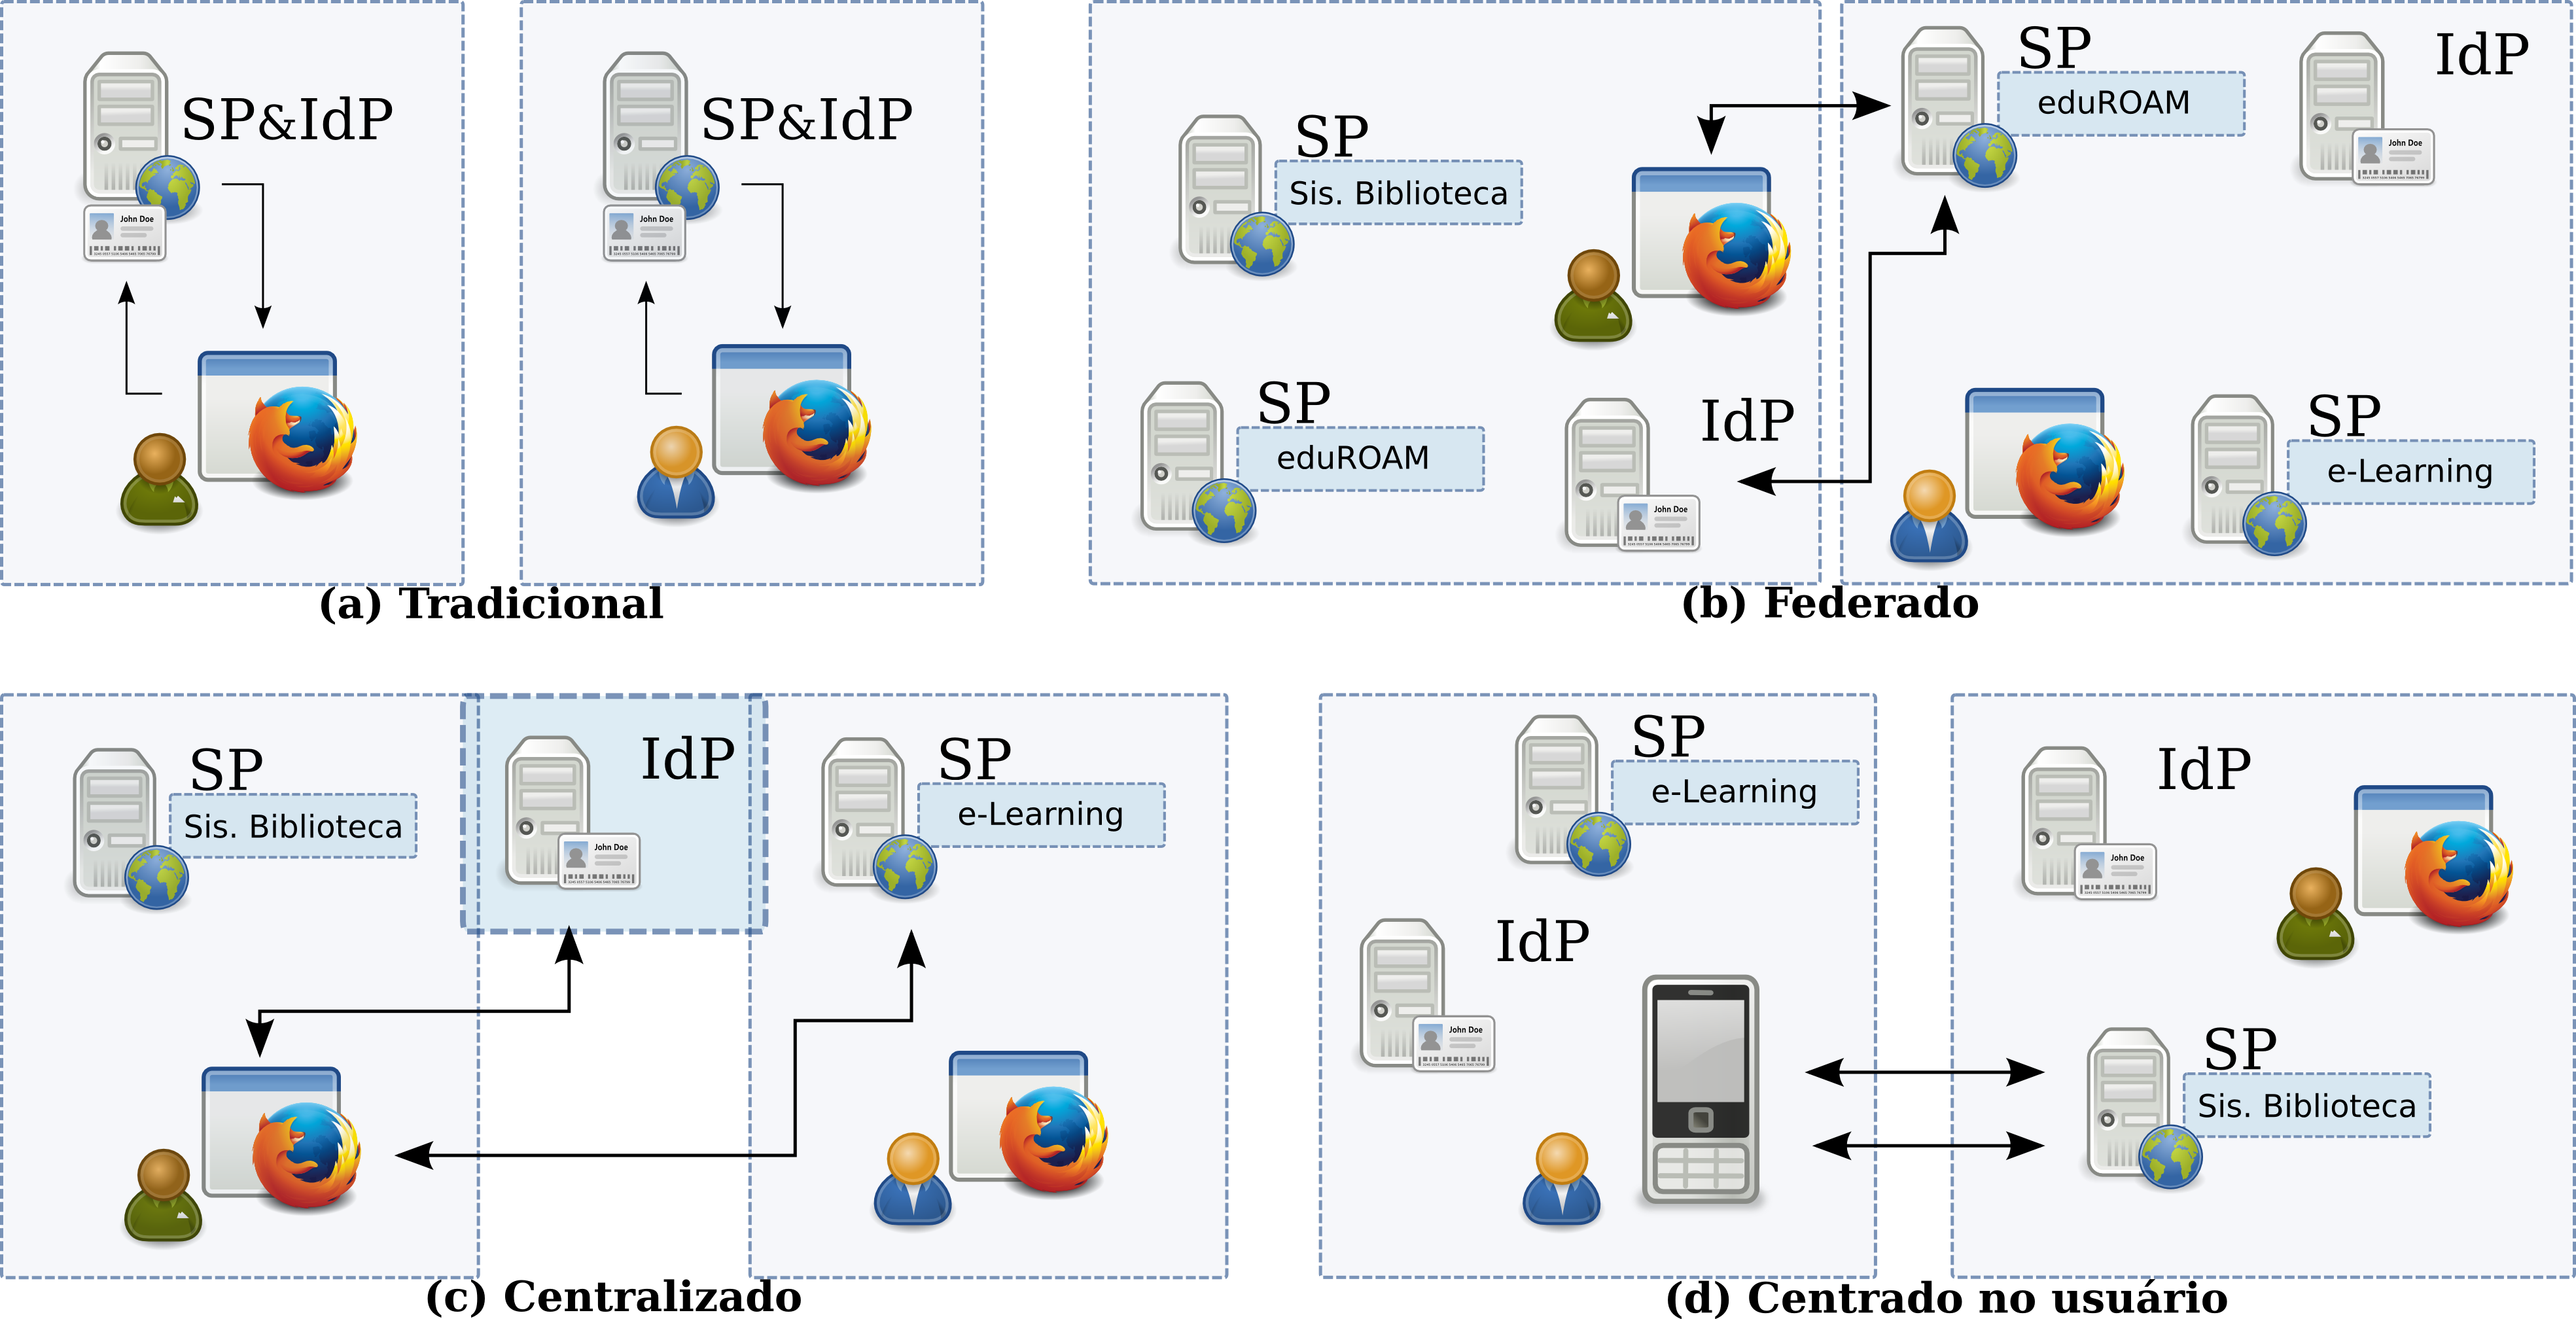
\includegraphics[width=1\textwidth]{figuras/modelos-gid.png}
 \caption{Modelos de Gestão de Identidade.}
 \label{fig_1}
\end{figure}

Dentre os modelos apresentados, é possível realizar algumas considerações quanto as suas características, por exemplo o modelo tradicional é amplamente utilizado nos atuais sistemas computacionais presentes na Internet. No entanto, apesar de ser amplamente utilizado seu uso tende a ser custoso tanto para o usuário quanto para os provedores de serviços. Implicando que os usuários possuam múltiplas identidades para interagir entre os diferentes serviços, como o servidor de e-mails, \textit{site} de notícias, livrarias, e outros. Cada provedor de serviços pode exigir um conjunto próprio de atributos para compor a identidade digital do usuário. Por outro lado, um conjunto comum de atributos pode ser exigido por diversos provedores de serviços, como nome da conta, senha, endereço, data de nascimento, etc. \cite{mello:09}.

O modelo centralizado trata destes problemas apontados sobre o modelo tradicional. O modelo centralizado fundamentalmente tem o compartilhamento de identidades dos usuários entre os provedores de serviços e no conceito de autenticação única (SSO), porém todas as identidades estão centralizadas num único  provedor de identidade, que detém o poder de todas as identidades, e podendo gerar discordâncias entre confiabilidade do uso destas pelo IdP \cite{wangham:10b}.

O modelo de gestão identidades federadas é uma abordagem que visa otimizar a troca de informações relacionadas a identidade por meio de relações de confiança construídas nas federações \cite{camenisch:07}. Os acordos estabelecidos entre provedores de identidades e de serviços garantem que identidades emitidas em um domínio sejam reconhecidas por provedores de serviços de outros domínios e o conceito de autenticação única é garantido mesmo diante de diferentes domínios \cite{wangham:10b}.

As principais propostas e implementações do modelo centrado no usuário fazem uso de um dos modelos apresentados anteriormente, sendo o modelo de identidade federadas o mais usado. O usuário se autentica neste dispositivo físico e cabe a este liberar as informações do usuário para cada provedor de serviços que o usuário acessar, respeitando totalmente as preferências de privacidade do usuário \cite{wangham:10b}.

\section{Especificações SAML}
\label{s_c2_saml}

A \acf{SAML} é uma especificação que define uma infraestrutura para troca de informações seguras da autenticação do usuário, seus direitos e atributos entre parceiros (instituições) na rede de computadores. A especificação SAML é elaborada pelo \ac{SSTC} que faz parte da \ac{OASIS}. A especificação SAML apresenta informações de segurança na forma de asserções (declarações). A especificação SAML define as regras e a sintaxe para geração, requisição, transferências e uso dessas asserções \cite{wangham:10b, oasis:08}.

As mensagens SAML são codificadas em arquivos XML que geralmente são incorporados em outras estruturas para o transporte, como por exemplo, o HTTP POST ou mensagens \ac{SOAP} codificadas. Esse tipo de transporte é denominado na especificação como \textit{binding}. A especificação SAML fornece um conjunto base de perfis para o uso de afirmações e protocolos, visando possibilitar a interoperabilidade no uso dos recursos SAML \cite{oasis:08, macaneiro:13}.

Atualmente, a especificação SAML está na versão 2.0 (lançada em 2005) e é o padrão mais adotado que concretiza o modelo de identidades federadas. Os sistemas de gerenciamento de identidades que utilizam a especificação SAML, o fazem por funcionalidades que estão disponíveis no padrão. A especificação SAML é utilizada de diferentes maneiras, as mais relevantes estão descritas em \cite{oasis:08}, tais como:

\begin{itemize}
 \item Web SSO -- a SAML possibilita o SSO por meio da comunicação de uma asserção de autenticação em um primeiro local para um segundo local que confia na origem da autenticação;
 \item Autorização baseada em atributos -- a especificação SAML permite a autorização baseada em atributos para comunicar informações de uma identidade entre diferentes \textit{web sites}, possibilitando desta forma apoio em algumas transações;
 \item Segurança em Serviços Web -- as asserções SAML podem ser usadas dentro das mensagens SOAP, afim de realizar operações com segurança de informações e identidade entre agentes em um serviço \textit{web}.
\end{itemize}

A especificação SAML é composta por alguns componentes que funcionam como blocos que podem ser combinados em configurações diferentes para suportar implementações de cenários diferentes. Os componentes primeiramente permitem transferência de identidade, autenticação, atributos e informações de autorização entre provedores de identidades e de serviços que possuem uma relação de confiança estabelecida. O núcleo da especificação SAML define a estrutura e o conteúdo das asserções e mensagens de protocolo usado para transferir essas informações \cite{oasis:08}.

\subsection{Componentes SAML}
\label{ss_c2_comp_saml}

Segundo \cite{oasis:08}, a especificação SAML é composta por componentes responsáveis por informações específicas, protocolos utilizados para troca dessas informações assim como os tipos de ligações que podem ser realizadas para o estabelecimento da comunicação entre elementos de uma federação.

A SAML define três tipos diferentes de declarações de afirmações que podem ser criadas por uma autoridade SAML. A estrutura e o conteúdo de uma asserção são definidos por meio de um esquema XML.

A asserção (\textit{assertion}) é usualmente criada por uma parte declarante (\textit{asserting party}) baseada em uma requisição da parte confiante (\textit{relying party}). No entanto, sob certas circunstâncias a asserção pode ser encaminhada para um parte confiante mesmo se não foi solicitada. Uma asserção é um pacote de informação que fornece uma ou mais declarações feitas por uma autoridade SAML. Uma asserção é composta basicamente por um conjunto de informações que são, a entidade da asserção, as condições usadas para validar a asserção e as declarações sobre o sujeito. Uma asserção pode conter três tipos de declarações:

\begin{itemize}
 \item Autenticação -- são geradas pela entidade que autentica o usuário. Possuem pelo menos o método de autenticação e de data e hora da autenticação;
 \item Decisão de autorização -- que especifica as permissões que o usuário tem no sistema, e que pode ser autorizada ou negada;
 \item Atributos -- que contêm informações específicas do usuário.
\end{itemize}

Os protocolos (\textit{protocols}) são mensagens de solicitações e respostas que os provedores de serviços podem utilizar. Os protocolos descritos na especificação SAML são:

\begin{itemize}
 \item protocolo de pedidos de autenticação;
 \item protocolo de consulta e pedido de asserção;
 \item protocolo para encerramento de sessão;
 \item protocolo para resolução de artefatos;
 \item protocolo de gerenciamento de identificador de nome;
 \item protocolo de mapeamento de identificador de nome.
\end{itemize}

As ligações (\textit{bindings}) SAML, são utilizadas pelos protocolos para transporte de mensagens entre as partes do sistema usando padrões de comunicação já estabelecidos. Na versão 2.0 da SAML estão disponíveis diversas ligações, dentre estas as mais comuns são:

\begin{itemize}
 \item HTTP \textit{Redirect Binding} -- o \textit{binding} HTTP \textit{Redirect} fornece um meio para transmitir asserções SAML dentro da URL de uma solicitação HTTP. Esta opção pode ser utilizada quando não é possível um caminho direto entre um provedor de identidade e um provedor de serviços. Neste caso a mensagem SAML será transportada de maneira indireta, normalmente, via o navegador web do usuário final;
 \item HTTP POST \textit{Binding} -- nesse modelo de \textit{binding}, as mensagens SAML são transmitidas dentro do conteúdo de um formulário HTML, utilizando do método HTTP POST para postar o SAML em um provedor de serviços;
 \item HTTP \textit{Artifact Binding} -- este modelo de \textit{binding} denominado de “Artefato HTTP SAML” fornece um mecanismo que permite a comunicação por intermédio de um agente do usuário HTTP intermediário. Esta ligação tem o objetivo de reduzir o fluxo de mensagens por meio do SAML;
 \item URI \textit{Binding} -- este modelo de \textit{binding} possibilita que uma asserção SAML específica seja repassada ao provedor de serviço por intermédio de uma HTTP URI;
 \item SOAP \textit{Binding} -- o SOAP é um protocolo de comunicação baseado no formato XML. É um protocolo simples, extensível e flexível, desenvolvido como um padrão W3C, importante no desenvolvimento de aplicações para permitir comunicação entre programas pela internet.
\end{itemize}

Os perfis (\textit{profiles}) SAML possibilitam que os protocolos do SAML e suas asserções trabalhem em fluxos de dados específicos, por exemplo, com a finalidade de promover a funcionalidade de gerenciamento de identidades e autenticação única (SSO). Existem também perfis de atributos (\textit{Attribute Profiles}) que não se referem a nenhuma mensagem de protocolo ou ligação, que definem como realizar a transmissão de informações de atributos usando asserções, de forma que se enquandre em usos comuns para diferentes tipos de ambientes (ex. X500, LDAP, DCE).

Na figura \ref{fig_2} é possível visualizar a pilha de componentes SAML conforme descritas anteriormente.

\begin{figure}[!ht]
 \centering
 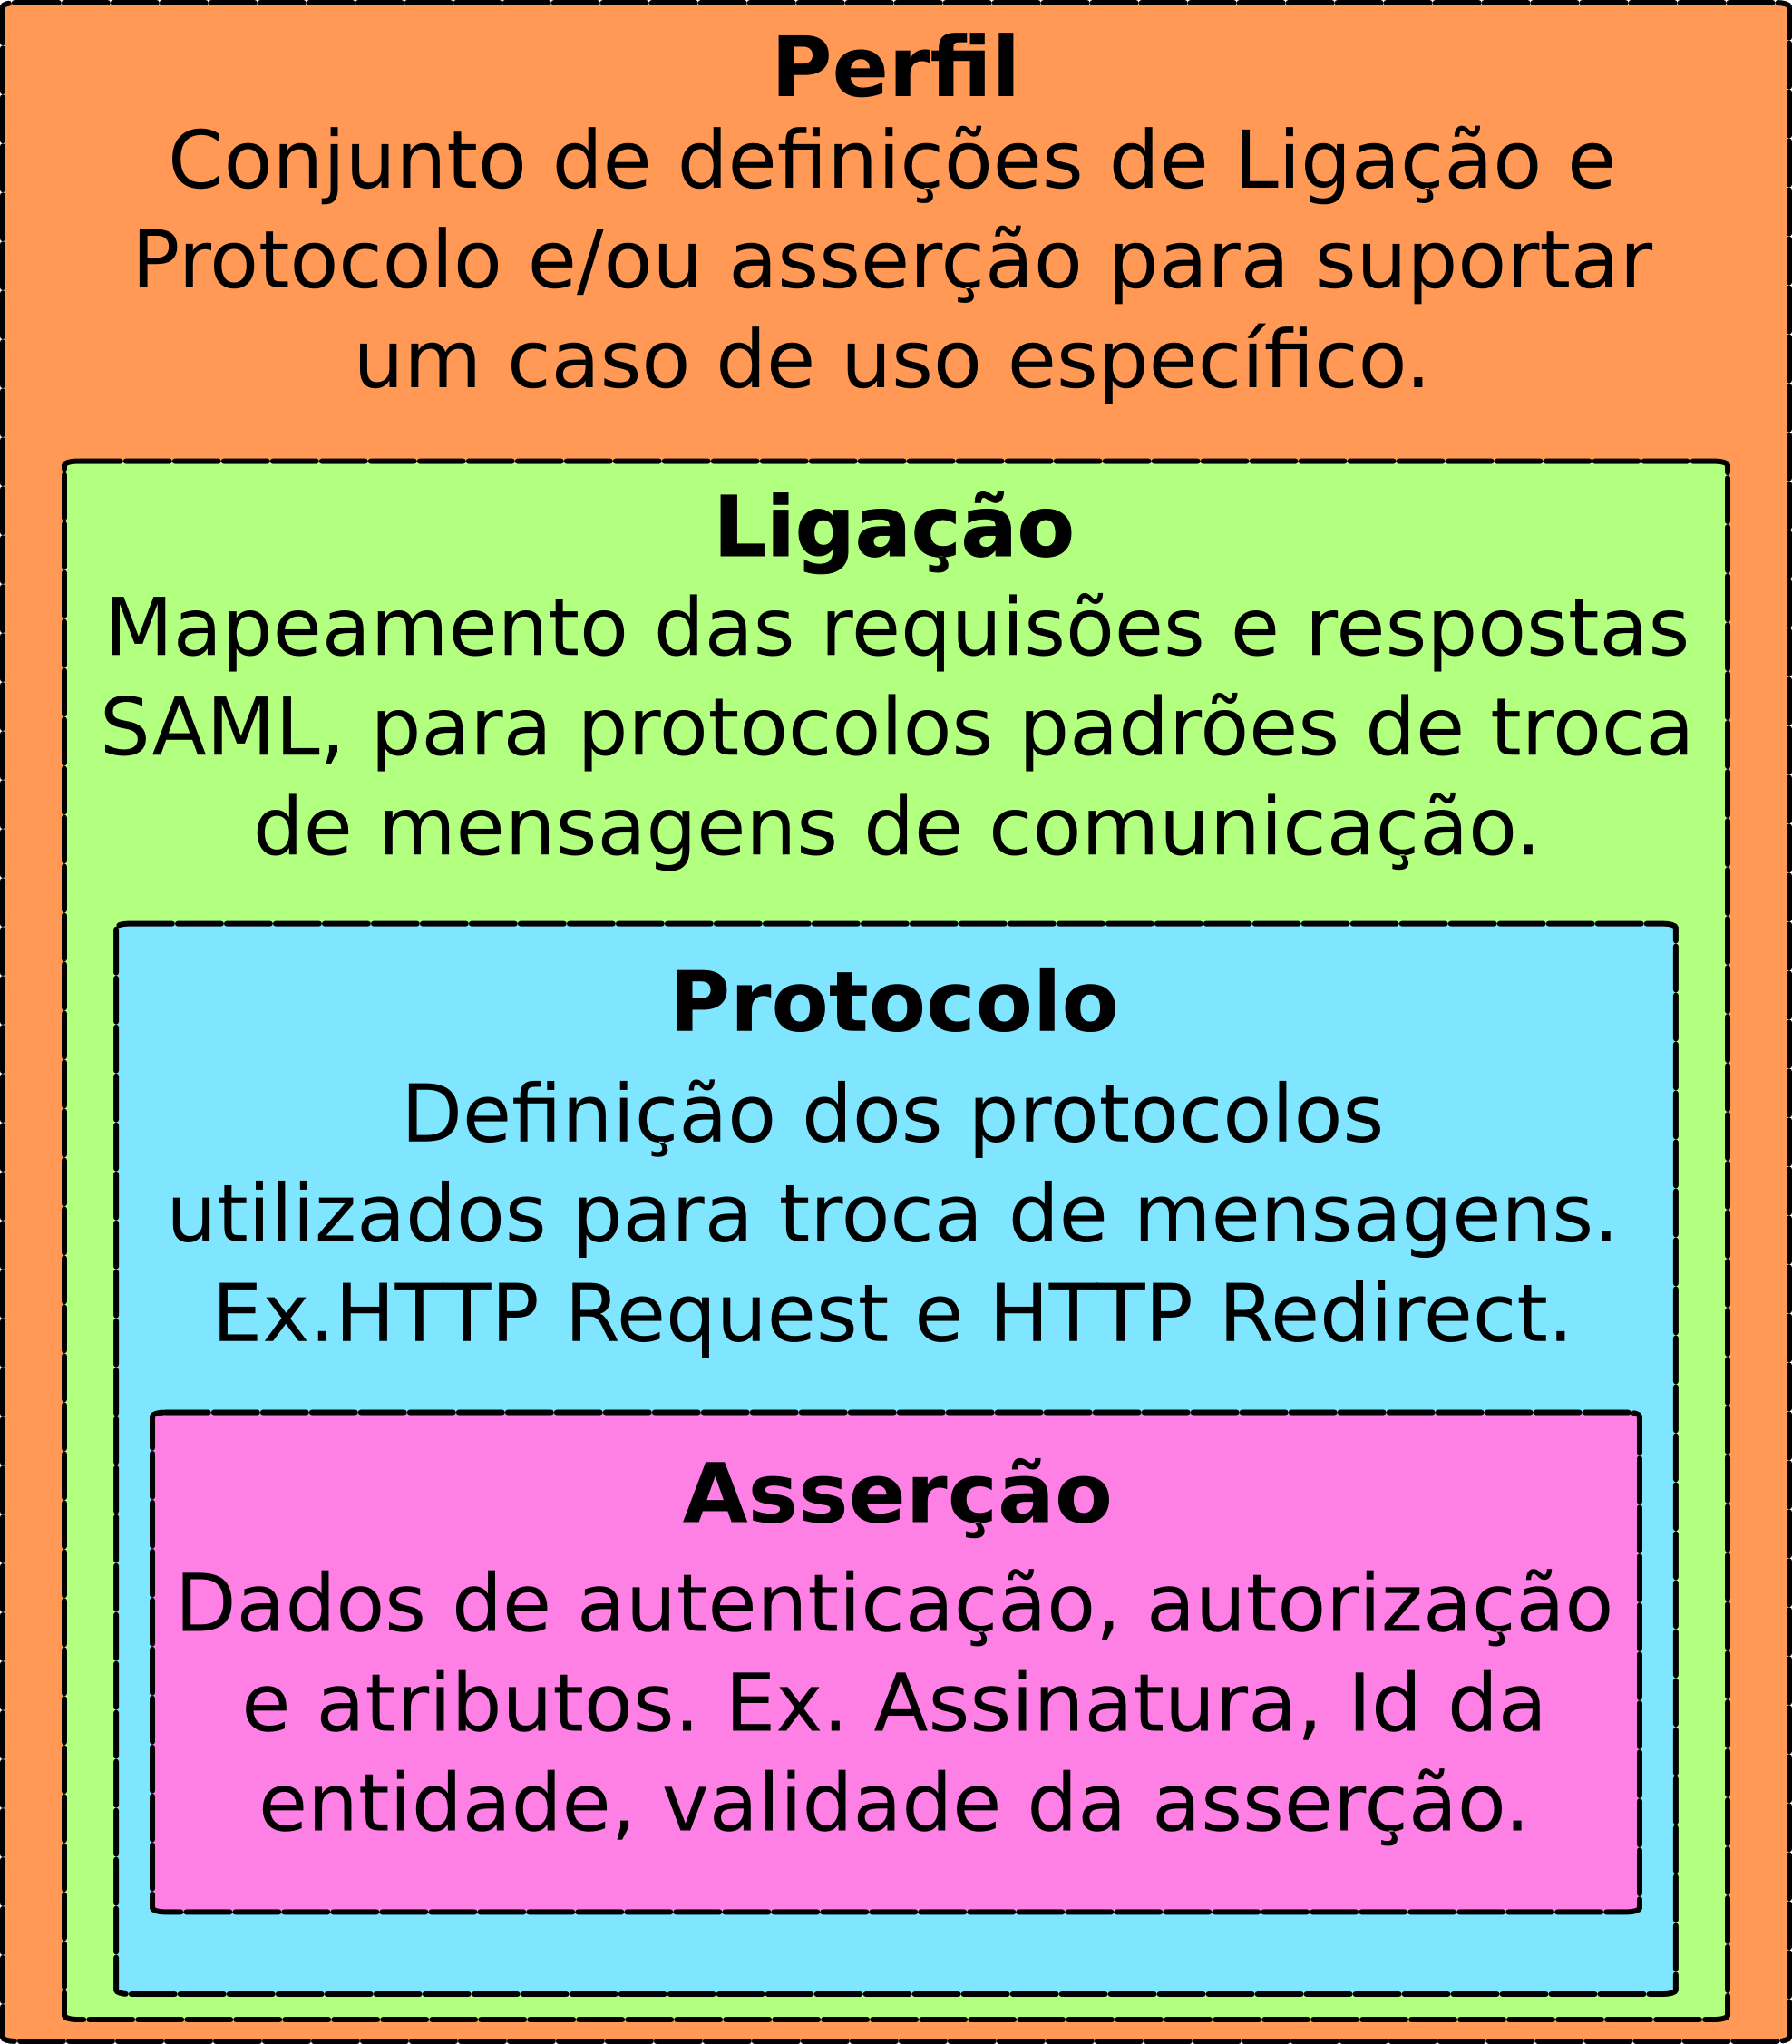
\includegraphics[width=0.6\textwidth]{figuras/pilha-saml.png}
 \caption{Pilha de componentes SAML.}
 \label{fig_2}
\end{figure}

Dois outros componentes bastante utilizados para composição de ambientes SAML, são:

\begin{itemize}
 \item Metadado -- que define como informar e compartilhar informações entre entidades SAML e papéis (como IdP, SP, etc.). O metadado contém informações sobre ligações SAML, identificadores de identidade, protocolos de transportes suportados, certificados digitais e chaves criptográficas; e
 \item Contexto de Autenticação -- em inúmeras ocasiões um provedor de serviço pode necessitar de informações detalhadas referente ao mecanismo de autenticação que é empregado pelo provedor de identidade do usuário. O contexto de autenticação SAML é usado para comunicação entre o provedor de serviços e o de identidades, permitindo ao primeiro solicitar uma forma específica de autenticação e ao segundo permitir o acesso do usuário em seus serviços \cite{oasis:08}.
\end{itemize}

\section{Framework Shibboleth}
\label{s_c2_framework}

O termo ``shibboleth'' denota uma palavra usada para distinguir pessoas de grupos distintos. A origem do termo remete ao velho testamento (Juízes, 12:1-15), onde ele foi usado para distinguir duas tribos semitas, os gileaditas e os efremitas, que travaram uma grande batalha. O gileaditas, vencedores, bloquearam a passagem do Jordão para evitar que os efremitas sobreviventes pudessem escapar. As sentinelas exigiam que todos o passante dissesse ``shibboleth''; como os efremitas não tinham o fonema \/x\/ em seu dialeto, só conseguiam pronunciar ``siboleth'' (com \/si\/ na primeira sílaba), eram identificas e executados \cite{moreira:11}.

O projeto \textit{Shibboleth} \cite{scavo:05} foi uma iniciativa do consórcio americano Internet2\footnote{http://www.internet2.edu/} que teve como principal objetivo lançar uma implementação de código aberto, baseada em padrões abertos, para tratar desafios relacionados ao gerenciamento de identidades e controle de acesso em instituições acadêmicas \cite{wangham:10a}.

O projeto \textit{Shibboleth} teve inicio em 2000 no comitê \ac{MACE}. O projeto do \textit{framework} se prolongou por um ano.  O \textit{framework} Shibboleth 1.0  foi lançado em Julho de 2003, em Agosto de 2005 foi lançado a versão 1.3, e por último (até ao momento) foi lançado a versão 2.0 em Março de 2008 \cite{manuel:09}. Já existem \textit{cases} oficiais de desenvolvimento de uma nova versão\footnote{http://shibboleth.net/documents/business-case.pdf}, com melhorias e novas implementações.

Com o amadurecimento do \textit{framework} Shibboleth, constata-se que este provê um sistema de gerenciamento de identidades federadas possível de ser adotado não só no âmbito acadêmico, mas também no governamental, e privado (comércio eletrônico).

Uma federação \textit{Shibboleth} é composta por um grupo de organizações e tem como princípio um conjunto de práticas comuns e de mecanismos de segurança e permissões previamentes definidas o que permite a participação \cite{carmody:05}.

O framework está fundamentado sobre padrões abertos como o XML e a SAML e provê uma forma fácil para que aplicações \textit{web} usufruam das facilidades providas pelo modelo de identidades federadas, como o conceito de autenticação única (SSO) e a troca segura de atributos dos usuários por todos provedores de serviços que compõem a federação \cite{wangham:10b}.

\subsection{Esquema brEduPerson}
\label{ss_c2_breduperson}

O \textit{framework} Shibboleth provê suporte a uma classe de atributos (\textit{Object Class}) chamado \textit{eduPerson}, que é um esquema LDAP, originalmente desenvolvida por \cite{internet2:08} baseado nas RFCs 2256\footnote{https://www.ietf.org/rfc/rfc2256.txt} e 2798\footnote{https://www.ietf.org/rfc/rfc2798.txt} \cite{wahl:97, smith:00}, respectivamente. É um conjunto padrão de atributos de identidades comuns para federações acadêmicas. Esta classe define quais atributos, informações, do usuário são necessárias para um funcionamento harmonioso entre IdP e SP dentro do escopo de uma instituição acadêmica. 

Usando como base este conjunto de atributos \textit{eduPerson} a RNP propôs uma adaptação deste esquema para as universidades e instituições brasileiras, e o denominou \textit{brEduPerson}. A gestão do esquema brEduPerson se dá conforme a figura \ref{fig_3}.

\begin{figure}[!htpb]
 \centering
 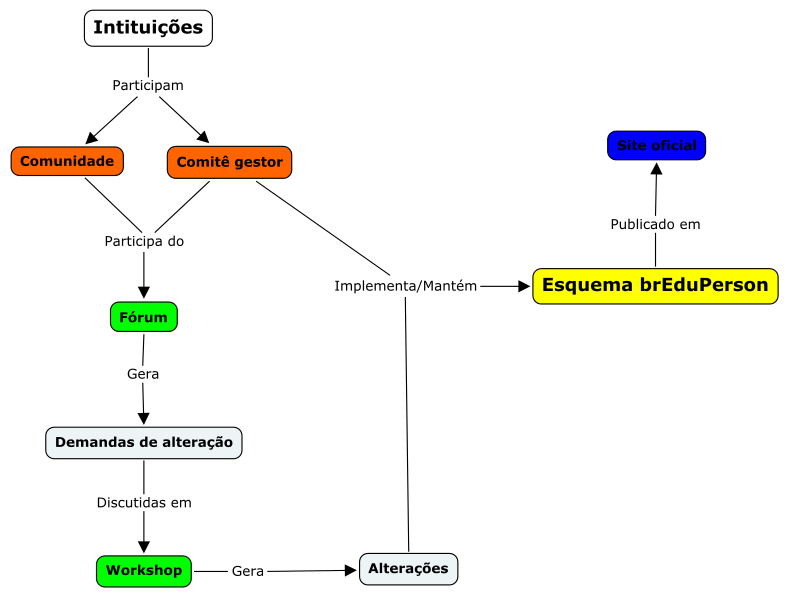
\includegraphics[width=0.8\textwidth]{figuras/gestao-breduperson.png}
 \caption{Gestão do esquema brEduPerson. Fonte: Esquema brEduPerson.}
 \label{fig_3}
\end{figure}

O esquema \textit{brEduPerson} visa complementar o conjunto original de esquemas que descrevem informações sobre pessoas, o \textit{inetOrgPerson}, o \textit{eduPerson} e o esquema \ac{SCHAC} definido por \cite{terena:09}. Este esquema armazena informações específicas para a realidade do país, tais como informações genéricas de qualquer cidadão residente no Brasil, (como CPF, Endereço, Passaporte), informações gerais sobre os membros de uma instituição (e-mail, cargo entre outros) além de informações específicas sobre os funcionários e alunos destas instituições. Tendo estas características definidas a RNP define que 6 atributos são altamente recomendados, 10 são sugeridos e 25 são opcionais\footnote{http://wiki.rnp.br/download/attachments/41190038/BrEduPersonv1
0.pdf}.

\subsubsection{Estrutura do esquema brEduPerson}
\label{ss_c2_estrut_breduperson}

Para o uso de um esquema em instituições de ensino e pesquisa, é necessário modelar relacionamentos entre conjuntos de informações. É preciso poder capturar na estrutura de diretórios LDAP o fato de uma mesma pessoa poder desempenhar diferentes papéis, como de um aluno (que também pode estar desempenhando uma pesquisa), e a cada um dos quais está associada uma data de ingresso, um código de curso, uma matrícula, e outras informações, ou que uma mesma pessoa pode ter direito a vários números \acs{VoIP}, cada um deles com suas características \cite{rnp:09}. Para modelar esses relacionamentos, a RNP optou por usar uma solução hierárquica.

Os nós em um diretório LDAP formam uma árvore. Cada nó, independentemente de originar algum outro nó na árvore, é uma entrada com suas próprias informações (atributos). Esses nós são por vezes chamados de \textit{containers} na terminologia X.500.

O item principal (uma pessoa) tem uma ligação com uma instituição de ensino e/ou pesquisa com o qual se deseja relacionar as demais informações deste vínculo, este item será tratado como um \textit{container} e abaixo deste aparecerão nós com as informações relacionadas. As informações genéricas (nome, cpf, e-mail, tipo de vínculo, etc), aparecerão como entradas, sobre ela, pois cada pessoa pode ter diferentes vínculos com a instituição, como vínculo de estudante em curso, vínculo de funcionário, etc. Ainda, abaixo da entrada com dados gerais podem aparecer diversas entradas descrevendo telefones VoIP, dados biométricos, formas de contato, como e-mail, telefone pessoal etc \cite{rnp:09}.

\subsubsection{eduPerson e brEduPerson}
A classe de objetos \textit{eduPerson} foi criada no contexto do Projeto Internet2\footnote{https://www.internet2.edu} para descrever indivíduos da comunidade acadêmica. O nome \textit{brEduPerson} é utilizado para descrever a classe de objetos que representa um vínculo com a instituição por ser o objeto cujos campos mais se assemelham aos da classe \textit{eduPerson}. O \textit{eduPerson}, no entanto, supõe apenas uma entrada por pessoa, com campos multivalorados descrevendo, por exemplo, os diversos vínculos de um indivíduo com a instituição. Esse modelo não satisfez as necessidades da Federação CAFe, pois era necessário associar a cada vínculo existente (professor, estudante, funcionário, etc) outras informações, como a data de entrada e saída. No esquema \textit{brEduPerson}, tanto a entrada principal de cada indivíduo (de classe estrutural \textit{brPerson}) como cada entrada abaixo dessa que descreve um vínculo (de classe estrutural \textit{brEduPerson}) têm a classe \textit{eduPerson} como auxiliar, 
pois atributos gerais do indivíduo ficam na entrada principal enquanto que os atributos relativos a um de seus vínculos ficam na entrada específica de vínculo \cite{rnp:09}. Na figura \ref{fig_4} é possível visualizar a distribuição dos atributos de uma pessoa, e seus vínculos.

\begin{figure}[!htpb]
 \centering
 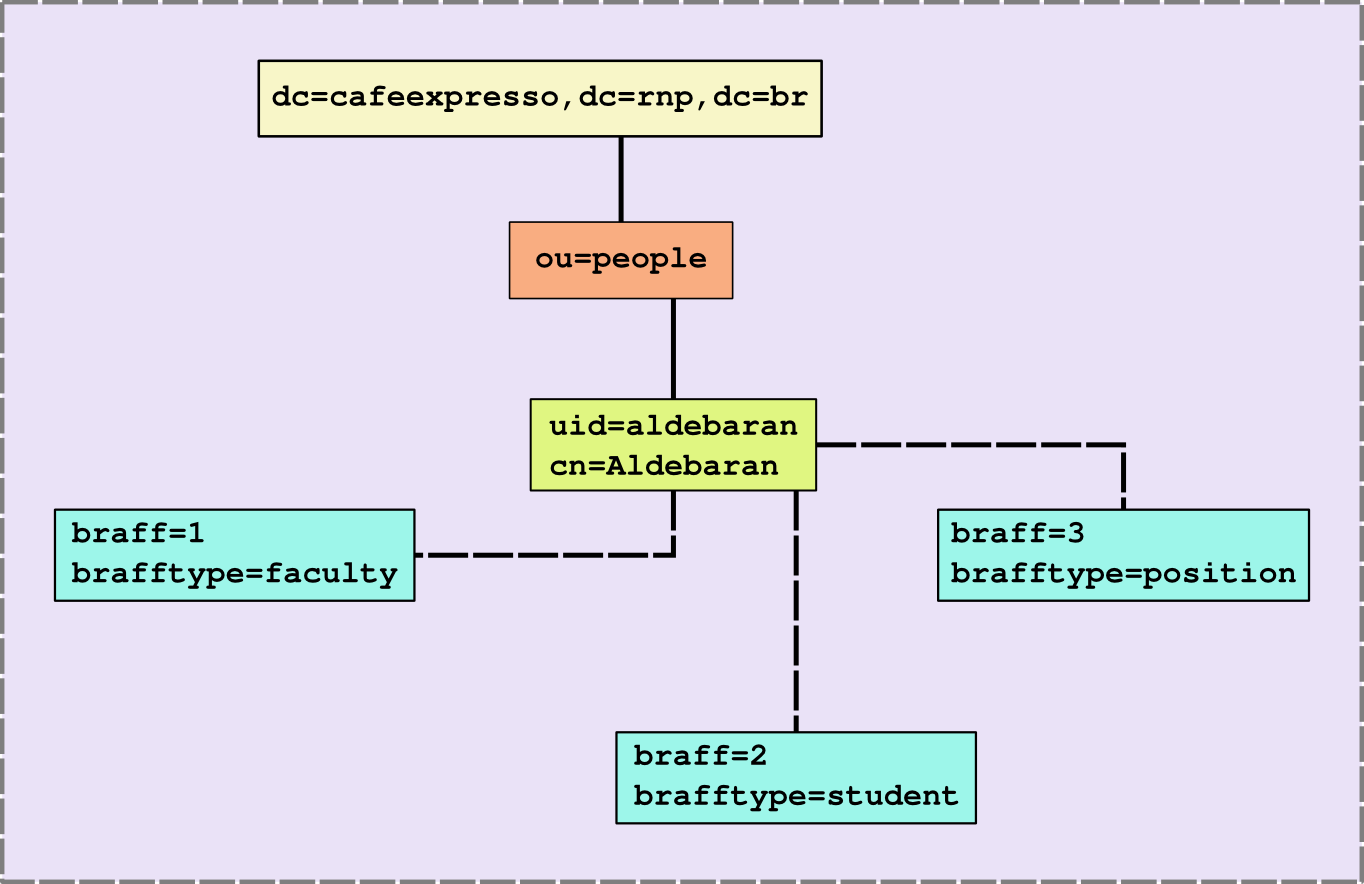
\includegraphics[width=0.8\textwidth]{figuras/arvore-breduperson.png}
 \caption{Árvore de atributos do brEduPerson.}
 \label{fig_4}
\end{figure}

Em um ambiente federado, a padronização destes atributos é fundamental para que provedores de serviços saibam quais atributos poderão requisitar e para que provedores de identidades saibam quais atributos deverão fornecer \cite{wangham:10a}.

\subsection{Provedores Shibboleth}
\label{s_c2_provedores}

O \textit{framework} Shibboleth é composto por dois provedores, que são chamados provedor de identidades, \acf{IdP}, e provedor de serviços, \acf{SP}. Estes são os principais compontes do framework. O IdP é a entidade responsável pelo gerenciamento das identidades dos usuários, seus atributos, gerenciamento da autenticação e declarações de atributos. Enquanto o SP é a entidade responsável pelo gerenciamento de segurança dos serviços disponibilizados, que, com base nas declarações de atributos recebidas do IdP, permite o acesso a estes serviços. A autorização para acesso ao serviço requisitado ainda passa por um conceito utilizado pelo \textit{framework} Shibboleth, dito contexto de segurança, que precisa ser estabelecido para um usuário, por meio da relação de confiança estabelecida entre SP e IdP, que permitirá o acesso seguro ao serviço \cite{kallela:08}.

No \textit{framework} Shibboleth, o processo de autenticação é executado na instituição de origem do usuário, por meio de seu provedor de identidades, fazendo uso dos mecanismos de autenticação presentes nesta instituição. A autenticação de usuários pode ser feita por meio de senhas, de tickets Kerberos, certificados X.509, entre outros mecanismos \cite{chadwick:09, wangham:10b}.

Um IdP é dividido em quatro subcomponentes \cite{scavo:05}:

\begin{itemize}
 \item Autoridade de autenticação -- serviço definido por meio da especificação SAML responsável por emitir pedidos de autenticação requisitado pela parte confiante (\textit{relying parties}), neste caso, o SP;
 \item Serviço de autenticação única (SSO) -- processo para a manipulação de requisições de autenticação de um usuário. Este componente obtém as requisições de asserção e gera um fomulário HTML que é redicionado para o SP;
 \item Serviço de resolução de artefatos -- um artefato é uma referência para uma asserção de autenticação. O SP define um perfil que utiliza a troca de asserções por referência, a resolução de artefatos (\textit{artifact binding}) é responsável por tratar estas requisições. O IdP ao invés de enviar a asserção de resposta de autenticação via navegador do usuário, envia uma asserção de referência a asserção expedida;
 \item Autoridade de atributos -- componente responsável pela emissão de asserções de atributos baseadas nas requisições dos provedores de serviços. Antes da edição de qualquer asserção, a autenticação e autorização das requisições recebidas precisam ser realidas.
\end{itemize}

Um SP assim como o IdP é formado por subcomponentes, são estes \cite{scavo:05}:

\begin{itemize}
 \item Recurso alvo --  os recursos Web são protegidos no SP por meio de serviços de Controle de Acesso, o que impede usuários não autenticados/autorizados de acessarem esses recursos;
 \item Serviço consumidor de asserção -- gerencia as funções de SSO no provedor de serviço. Processa a asserção de atributos recebida ou o artefato, podendo elaborar requisições de asserções de atributos adicionais, estabele contexto de segurança e redirecionada o usuário para o serviço em ambiente seguro;
 \item Requisitante de atributos -- realiza interações com a autoridade de atributos do IdP, para realizar trocas adicionais de atributos, uma vez que um contexto de segurança tenha sido estabelecido. Esse tipo de interação ocorre diretamente entre os provedores, por meio dos protocolos de ligação (\textit{binding}) SAML, e não utilizam o navegador Web do cliente.
\end{itemize}

Adicionalmente, um terceiro componente é especificado no \textit{framework} Shibboleth, o serviço de descoberta ou \acf{DS}. Na CAFe Expresso foi implantado dois tipos diferentes de DS, o \acf{WAYF} e o \acf{EDS}. Ambos os serviços, WAYF e EDS realizam o redirecionamento do usuário entre o provedor de serviços e o provedor de identidades. Uma vez que o provedor de serviço não sabe, nem tem obrigação de saber, qual o provedor de identidades que o usuário utiliza para validar seus credenciais de autenticação. O WAYF mantém uma base dos provedores utilizando metadados SAML, que além de realizar o estabelecimento de relação de confiança entre os provedores, provê o redirecionamento do usuário para seu provedor de identidade de origem \cite{shibb:05, kallela:08, wangham:10b}. O EDS no entanto permite o uso da mesma base disponibilizada pelo WAYF, porém o processo de redirecionamento do usuário entre SP, EDS e IdP é transparente para o usuário. Além do que, o EDS é embutido diretamente na página do SP, diminuindo 
ainda mais os redirecionamentos entre páginas \textit{web}.

\begin{figure}[!htpb]
 \centering
 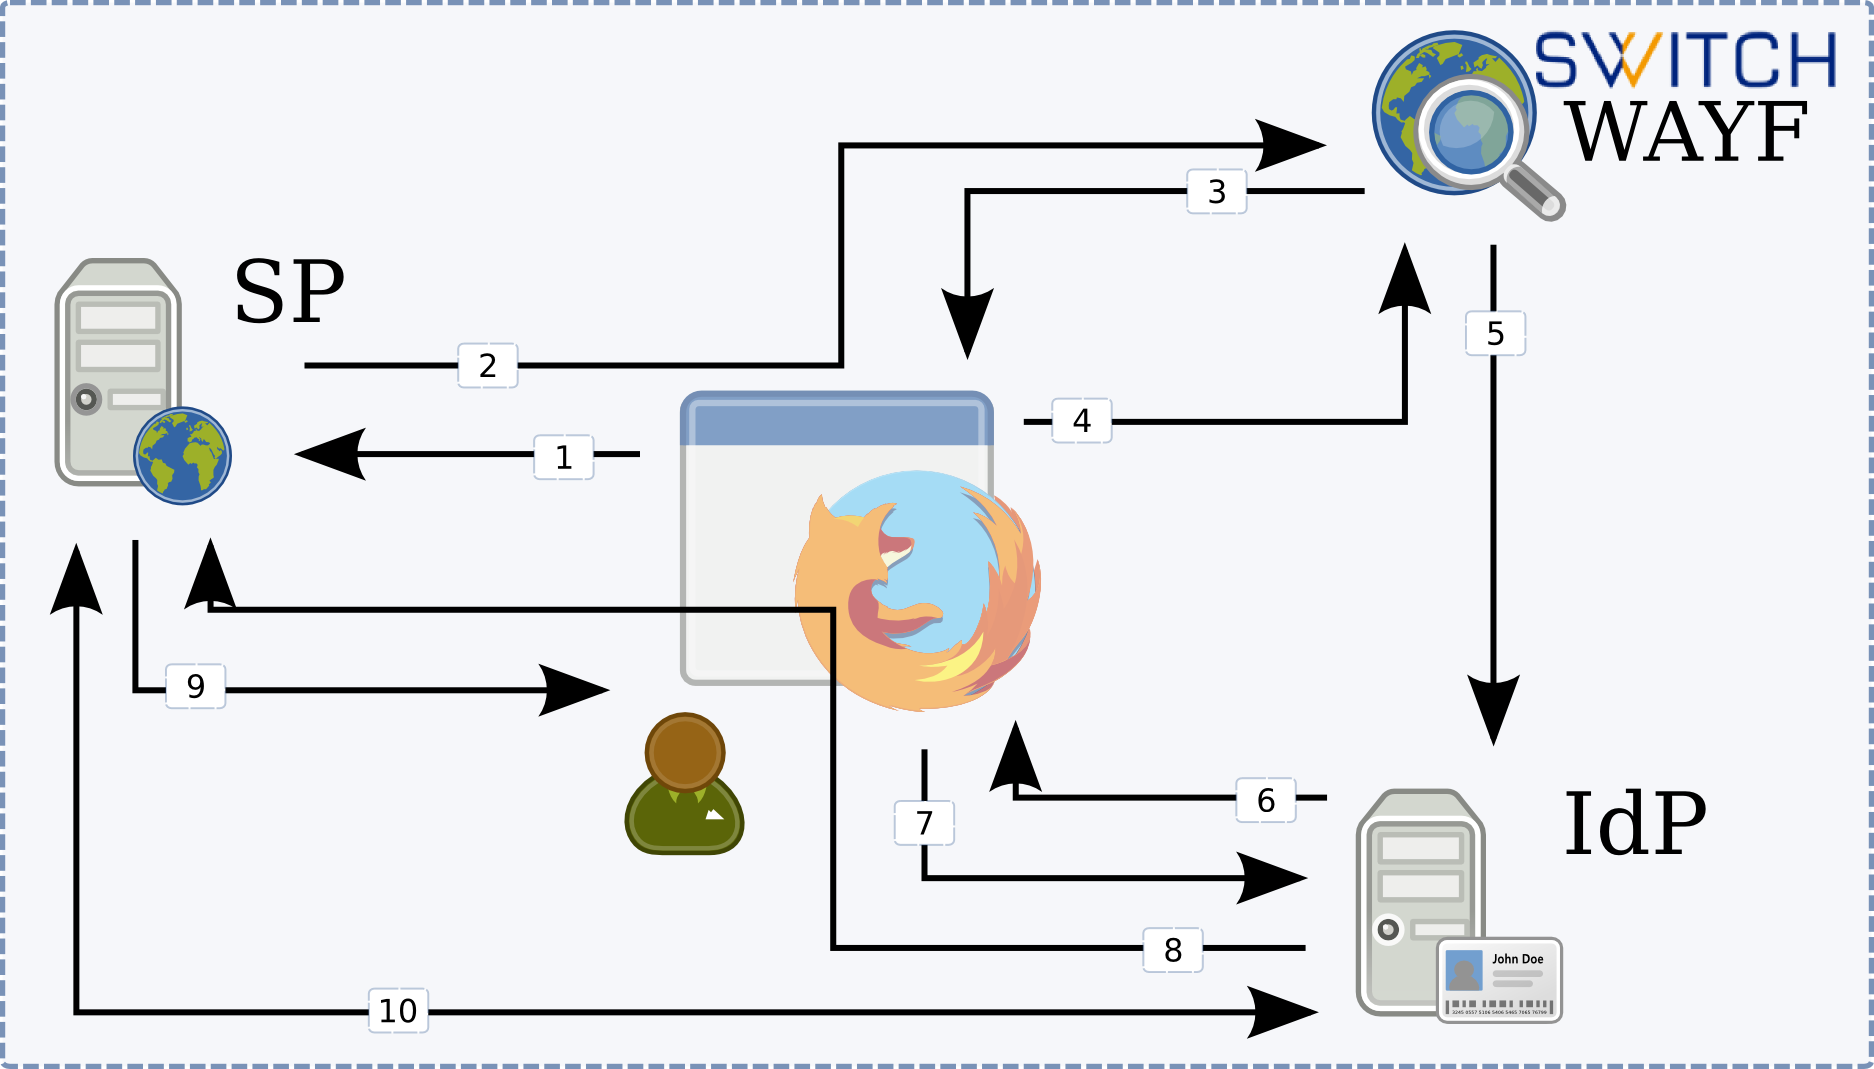
\includegraphics[width=0.8\textwidth]{figuras/fluxo-shibboleth.png}
 \caption{Fluxo de mensagens entre usuários e provedores Shibboleth.}
 \label{fig_5}
\end{figure}

A Figura \ref{fig_5} exemplifica o fluxo de mensagens trocadas entre os provedores quando um usuário realiza a requisição de um serviço a um provedor de serviços da federação, conforme descritos a seguir \cite{feliciano:11}:

\begin{itemize}
 \item Passo 1 -- O usuário através do navegador web solicita acesso a um serviço protegido por um provedor de serviços da federação;
 \item Passo 2, o provedor de serviços recebe a requisição e redireciona o navegador do usuário  para o serviço de descoberta ou DS;
 \item Passo 3, o DS apresenta uma lista de IdPs da federação;
 \item Passo 4, o usuário informa o seu provedor de identidades;
 \item Passo 5, o DS atualiza o cookie de sessão com as informações do IdP escolhido e redireciona o navegador do usuário para o IdP indicado;
 \item Passo 6, o serviço de SSO é requisitado no IdP escolhido e este adquire uma declaração de autenticação (asserção SAML) da Autoridade de Autenticação, que retorna a asserção SAML gerada para o navegador do usuário;
 \item Passo 7, o usuário fornece as suas credenciais por meio de uma mensagem HTTP POST para o IdP de origem;
 \item Passo 8, o IdP autentica o usuário e uma asserção SAML é retornada para o navegador do usuário e o serviço consumidor de asserção do SP processa a resposta da autenticação. O contexto de segurança é criado no SP e redirecionamento do usuário para o recurso solicitado;
 \item Passo 9, opcionalmente, o provedor de serviço pode enviar um pedido de atributos ao provedor de identidade do usuário;
 \item Por fim, no passo 10, o provedor de identidade retorna os valores dos atributos requisitados.
\end{itemize}
% ----------------------------------------------------------------------- %
% Arquivo: cap3.tex
% ----------------------------------------------------------------------- %
\chapter{Federação CAFe}
\label{c_cap3}

Em Julho de 2007 a RNP com a colaboração das instituições Cefet-MG, UFC, UFF, UFMG, e UFRGS, dentro do escopo do projeto e-AA: Infraestrutura de Autenticação  e Autorização Eletrônica tinha como objetivo criar condições necessárias para a implantação de uma comunidade acadêmica federada no Brasil. Uma federação acadêmica envolve instituições de ensino e pesquisa e permite que as pessoas vinculadas a estas instituições compartilhem informações e recursos e tenham acesso a serviços restritos, usando o vínculo institucional como critério básico para esse compartilhamento \cite{moreira:11}. A partir destes esforços surgiu a \acf{CAFe}.

A CAFe tem como objetivo congregar todas as universidades e instituições de pesquisa brasileiras. A metodologia adotada para construção da infraestrutura básica de federação consiste na utilização de padrões e soluções de software já disponíveis e adotados por outras federações, e da implementação e experimentação de ferramentas auxiliares para apoiar a implantação de provedores de identidades e de serviços. O projeto de criação da Federação CAFe inclui ainda o estudo, a proposição, a análise e a validação de políticas para regular o funcionamento da federação \cite{moreira:11}.

\section{Como funciona}
\label{s_c3_funciona}

As instituições pertencentes à CAFe podem atuar como provedores de identidade (IdP) ou como provedores de serviço (SP), ou ainda podem ter ambos os provedores dentro das suas dependências. As organizações usuárias da RNP que atuam como provedores de identidade têm atualmente um subsídio completo no preço associado ao uso do serviço da CAFe. Além disso, nenhum dos acordos atuais prevê qualquer custo para os provedores de serviço. A RNP é responsável pela gestão do serviço e por manter o repositório centralizado com dados sobre integrantes da federação \cite{rnp:13}.

A CAFe possibilita que cada usuário tenha uma conta única em sua instituição de origem, válida para todos os serviços oferecidos à federação, eliminando a necessidade de múltiplas senhas de acesso e processos de cadastramento. A relação de confiança entre instituições participantes da Federação permite que o usuário se autentique unicamente em sua instituição de origem, que fornece as garantias de autenticidade e credibilidade necessárias às demais \cite{rnp:13}.

Outro aspecto positivo é o controle sobre a privacidade dos dados. Ao invés de ter um cadastro individual em cada serviço, a federação permite que o provedor de identidade forneça ao provedor de serviço apenas o mínimo de informação necessária para o controle de autorizações. Isto pode variar da simples garantia de que aquele usuário é reconhecido e autenticado pela instituição até informações sobre seu status ou tempo de serviço junto a essa instituição. Os acordos firmados pelos provedores de serviço com a CAFe garantem que os dados serão usados apenas para os fins combinados\footnote{http://portal.rnp.br/web/servicos/beneficios}.

Diversos países já têm federações em funcionamento ou em implantação. Dentro das redes de instituições de ensino, os serviços de ensino a distância e atividades de colaboração estão entre os maiores beneficiários das infraestruturas oferecidas por federações \cite{rnp:13}.

\section{Serviços disponíveis}
\label{s_c3_servicos}

Alguns serviços disponíveis através da CAFe são:

\begin{itemize}
 \item video@RNP -- O portal de Vídeo Digital da RNP agrega três diferentes serviços (Vídeo Sob Demanda, Transmissão de Vídeo ao Vivo e Transmissão de Sinal de TV) e se integra ao conteúdo do serviço Videoaula@RNP;
 \item JEMS -- O Journal and Event Management System (JEMS) é um sistema para submissão, revisão, discussão e seleção de artigos para eventos científicos da Sociedade Brasileira de Computação (SBC), mantido pela Universidade Federal do Rio Grande do Sul (UFRGS). Seu principal objetivo é disponibilizar para acadêmicos participantes de eventos da SBC uma infraestrutura para envio de artigos e resumos para avaliação. Assim, é possível a análise de tais documentos por parte da organização do evento e a decisão de quais deles serão selecionados para participação;
 \item GENI -- O \textit{Global Environment for Network Innovations} (GENI\footnote{https://portal.geni.net/}) é um portal de infraestrutura de pesquisa patrocinado pela National Science Foundation, órgão dos Estados Unidos de fomento ao desenvolvimento científico. O portal disponibiliza um ambiente laboratorial para redes e sistemas distribuídos para ensino e pesquisa com múltiplos testbeds. O laboratório virtual possibilita pesquisas sobre o futuro das redes de grande porte, criando oportunidades de compreensão, inovação e transformação das redes globais e suas interações com a sociedade;
 \item RedCLARA -- Os serviços que operam sobre a infraestrutura de Internet Avançada de RedCLARA\footnote{http://www.redclara.net/index.php} são destinados a promover o desenvolvimento de iniciativas de colaboração científica e acadêmica na América Latina, oportunidades reais para pesquisadores, cientistas e acadêmicos da região;
 \item Gisela -- O Gisela Science Gateway é um portal de aplicações científicas do projeto Grid Initiatives for e-Science virtual Communities in Europe and Latin America (GISELA), que funciona como uma interface para um ambiente de grid;
 \item Atlases -- O Atlases é uma biblioteca de imagens de patologia em alta resolução. É voltado para estudantes de Medicina e profissionais da área médica;
 \item PADBR -- A grade computacional PADBR oferece acesso integrado aos recursos de alto desempenho distribuídos geograficamente entre os Centros Nacionais de Processamento de Alto Desempenho (CENAPADs) geograficamente distribuídos. São nove unidades, operadas respectivamente pela UFRGS, UFMG, UFC, UNICAMP, UFRJ, UFPE, INPE, INPA e LNCC. Esse último coordena o sistema por delegação do Ministério da Ciência, Tecnologia e Inovação (MCTI).
\end{itemize}

Todos os serviços descritos acima estão disponíveis para acesso gratuito. Além destes, muitos outros serviços podem ser utilizados através do acesso pela CAFe. Uma lista de serviços pode ser vista no \textit{site} da CAFe, em serviços disponíveis\footnote{http://portal.rnp.br/web/servicos/servicos-disponiveis}

\section{Acordos internacionais}
\label{s_c3_acordos}

A disponibilização, ou criação de novas, infraestruturas de autenticação e autorização federadas para as suas comunidades acadêmicas está se tornando uma prática comum em vários países. O próprio Shibboleth, software utilizado na CAFe, foi desenvolvido pela Internet2 para dar suporte à criação da Federação InCommon\footnote{http://www.incommonfederation.org/}. Tipicamente, as iniciativas de criação de infraestruturas federadas são coordenadas pelas redes nacionais de ensino e pesquisa, \ac{NREN}, como a RNP. A CAFe se tornou um projeto pioneiro no Brasil e alcançou acordos internacionais, permitindo e à integração entre diferentes federações do Mundo \cite{rnp:13}.

\subsection{EduGAIN}
\label{ss_c3_edugain}

A Comunidade Acadêmica Federada (CAFe) integra, desde dezembro de 2012, o serviço eduGAIN\footnote{http://www.geant.net/service/edugain/pages/home.aspx}, que reúne, em uma rede de confiança, as federações de gestão de identidade sócias da GÉANT\footnote{http://www.geant.net/pages/home.aspx} (Rede de pesquisa pan-européia). A organização é uma rede de alta capacidade que engloba mais de três mil instituições de ensino e pesquisa em 32 países, através de 28 redes nacionais e regionais de ensino e pesquisa.

\begin{figure}[!htpb]
 \centering
 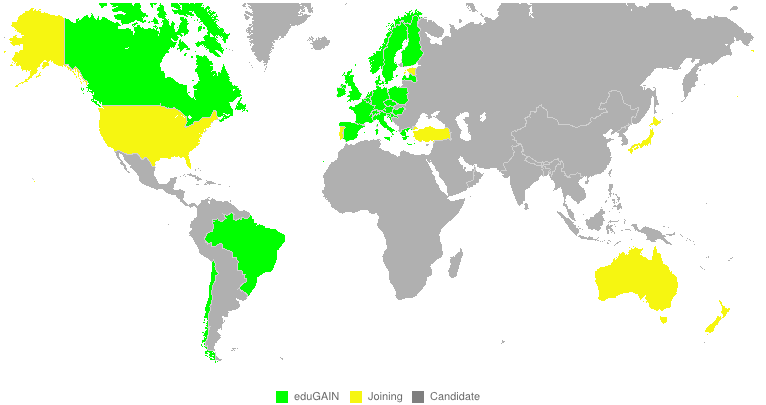
\includegraphics[width=1\textwidth]{figuras/edugain2.png}
 \caption{Mapa de países com federações participantes da EduGAIN. Fonte: EduGAIN (http://edugain.org/technical/status.php)}
 \label{fig_6}
\end{figure}

Além do Brasil, representado pela CAFe, fazem parte da eduGAIN federações da Croácia, Finlândia, Hungria, Itália, Noruega, Espanha, Suécia e Suíça. Constam também na lista de candidatos a integrar a confederação os seguintes países: República Tcheca, França, Alemanha, Grécia, Letônia e Holanda. A CAFe foi, portanto, a primeira federação das Américas a fazer parte desta rede de confiança.

O principal benefício para os clientes da CAFe é a possibilidade de utilizar os diversos serviços disponibilizados pelas inúmeras organizações que integram eduGAIN.

\subsection{REFEDS}

Desde março de 2011, a CAFe integra o mapa das federações de identidade mundiais de educação e pesquisa mantido pela Research and Education Federations (REFEDS)\footnote{http://www.terena.org/activities/refeds}.

\begin{figure}[!htpb]
 \centering
 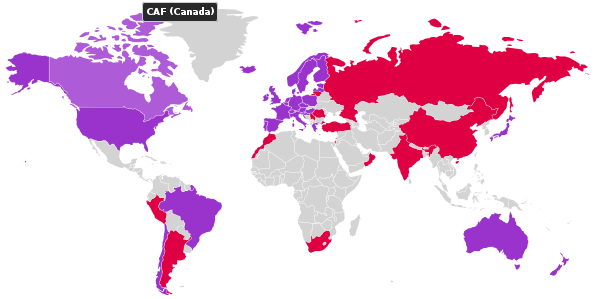
\includegraphics[width=1\textwidth]{figuras/cafe-refeds.png}
 \caption{Mapa de países com federações participantes da REFEDS. Fonte: REFEDS (https://refeds.org/resources/)}
 \label{fig_7}
\end{figure}

Assim, a CAFe se tornou a primeira federação da América Latina a ser reconhecida internacionalmente pela iniciativa, gerenciada pela \ac{TERENA}\footnote{http://www.terena.org/}, que articula as necessidades de federações de identidade para educação e pesquisa em todo o mundo.

Os participantes da REFEDS compartilham o interesse de desenvolver tecnologias, políticas e processos de gestão de identidade. Muitos destes representam redes nacionais de ensino e pesquisa, \ac{NREN}, como é o caso da RNP.
% ----------------------------------------------------------------------- %
% Arquivo: cap4.tex
% ----------------------------------------------------------------------- %
\chapter{Federação CAFe Expresso}
\label{c_cap4}

Para desenvolver pesquisas aplicadas na área de Gestão de Identidades é necessário que os experimentos sejam conduzidos em um ambiente que implemente uma federação em sua totalidade, no entanto montar tal ambiente depende do \textit{framework} escolhido \cite{wangham:13}. A complexidade e trabalho para implantar uma federação usando o \textit{framework} Shibboleth por exemplo, é muito alta. A Federação CAFe Expresso é uma resposta da RNP às necessidades de pesquisadores que atuam na área de gestão de identidades federadas \cite{wangham:13}.

Desde 2009, a RNP disponibiliza o serviço da \ac{CAFe} às suas organizações usuárias. Por meio da CAFe, um usuário mantém todas as suas informações na sua instituição de origem e pode acessar serviços oferecidos pelas instituições que participam da federação acadêmica.

A federação CAFe é um ambiente de produção, ou seja, nesta federação não deve ser permitida a realização de experimentos, assim pesquisadores que fazem prospecções tecnológicas e pesquisas científicas em gestão de identidade necessitam montar sua própria federação de testes para que possam conduzir seus projetos e experimentos.

Motivada por esta necessidade, a RNP criou em 2013 o projeto \acf{GId Lab}\footnote{http://wiki.rnp.br/display/gidlab} que tem por objetivo disponibilizar para a comunidade acadêmica um ambiente virtual no qual os pesquisadores possam realizar testes com Infraestruturas de Autenticação e Autorização (IAA) e também Infraestruturas de Chaves Públicas (ICPs).

O projeto GId Lab é mantido pela RNP como plataforma de apoio aos pesquisadores brasileiros, principalmente os participantes do \ac{PGID} e dos \acp{GT} da RNP \cite{wangham:13}.

O projeto GId Lab provê a CAFe Expresso, uma Infraestrutura de Autenticação e Autorização que trata da especificação de uma federação para experimentos permitindo que desenvolvedores e pesquisadores de qualquer instituição de ensino do Brasil possam desenvolver serviços ou disponibilizar um provedor de identidade, tendo como base o \textit{framework} Shibboleth.

O projeto GId Lab provê ainda o \ac{SGCI}\footnote{https://projetos.labsec.ufsc.br/sgci} da \ac{ICPEdu}\footnote{http://www.rnp.br/servicos/icpedu.html}, um software desenvolvido para o âmbito acadêmico, em uso em diversas universidades e centros de pesquisas brasileiros, que permite a implantação e gerenciamento de \acp{AC} para emissão de certificados digitais. Este provê as funcionalidades necessárias para o gerenciamento de \acf{ICP} \cite{wangham:13}. No entanto essa parte não será coberta no referido trabalho.

O trabalho em questão foi desenvolvido dentro do escopo do projeto Gid Lab \cite{wangham:13} onde uma infraestrutura de \ac{GId} foi implantada, afim de facilitar o desenvolvimento de pesquisas na área de GId. No entanto o projeto GId Lab, é muito mais amplo que somente a infraestrutura de Gestão de Identidades Federadas usando o \textit{framework} Shibboleth, sendo assim, este trabalho em questão abordará somente uma parte do GId Lab.

\section{Visão geral da solução proposta}
\label{s_c4_visao}

A Figura \ref{fig_8} ilustra a infraestrutura de autenticação e autorização disponível dentro do GId Lab, assim como as máquinas virtuais que serão disponibilizadas para os pesquisadores interessados.

\begin{figure}[!htpb]
 \centering
 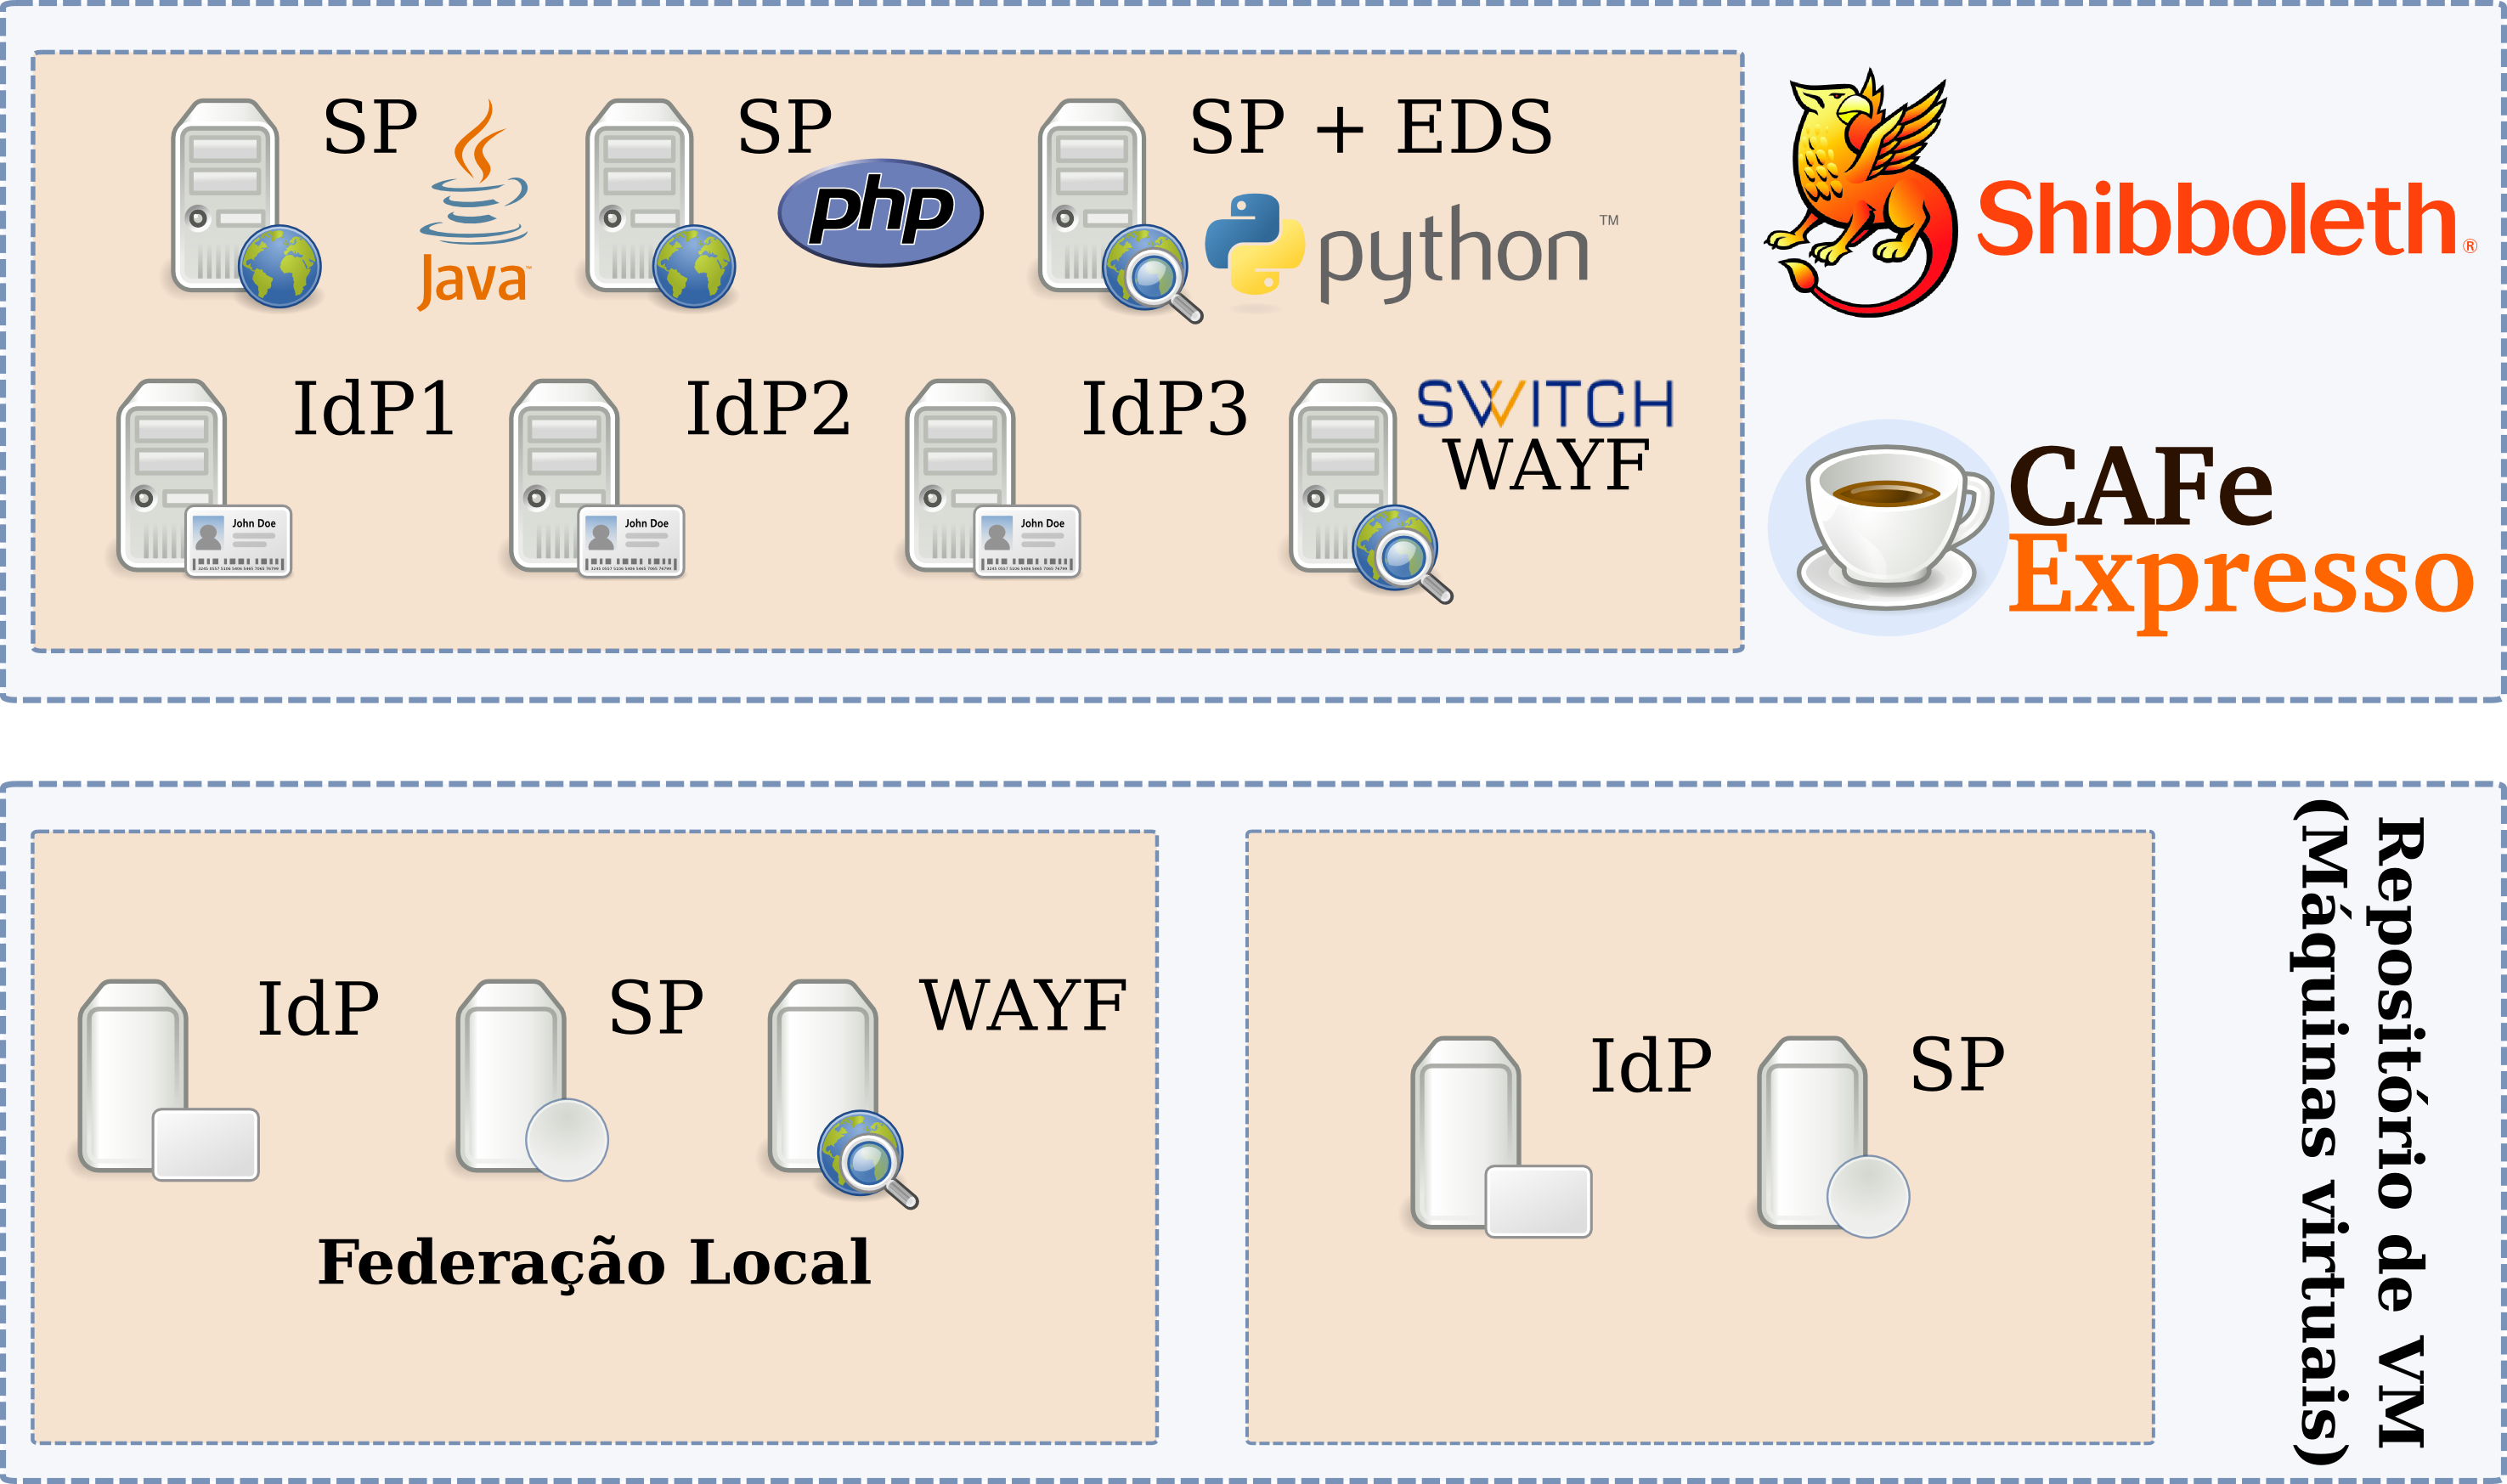
\includegraphics[width=1\textwidth]{figuras/infra-cafeexpresso.png}
 \caption{Estrutura da CAFe Expresso no GId Lab.}
 \label{fig_8}
\end{figure}

Dentro do contexto do projeto GId Lab a CAFe Expresso, irá oferecer dois IdPs alimentados com usuários com diferentes perfis e atributos, e dois SPs configurados para proteger aplicações web em PHP, Java e Python. Desta forma, pesquisadores poderão implementar suas soluções em uma dessas linguagens e só precisarão disponibilizá-las por meio destes SPs \cite{wangham:13}. Estes provedores de serviços e de identidades estão espalhados\footnote{http://wiki.rnp.br/display/gidlab/Infraestrutura} pelos \acp{PoP} da Rede Ipê\footnote{http://www.rnp.br/ipe/} da RNP \cite{wangham:13}.

Pretende-se ainda integrar aos IdPs da CAFe Expresso o módulo de consentimento do usuário, conhecido como \textit{uApprove}\footnote{http://www.switch.ch/aai/support/tools/uApprove.html}. Este módulo tem como objetivo informar ao usuário quais atributos estão sendo liberados para o SP, no momento que está sendo solicitado a autenticação do usuário no IdP da sua instituição e o encaminhamento, por meio da asserção de atributos SAML, para o SP no qual está sendo solicitado o serviço.

Conforme indicado na Figura \ref{fig_8}, o projeto GId Lab disponibiliza aos pesquisadores um repositório com máquinas virtuais (\acp{VM}. No repositório estará disponível duas possibilidades de ambiente para criar uma federação, o pesquisador poderá escolher criar uma federação local na instituição que contemplará um ambiente completo, com um IdP, um SP e um WAYF. Outra possibilidade, será as VMs com IdP ou SP pré-configurado, pronto para adesão na federação CAFe Expresso.

O serviço \acf{WAYF}, é um serviço de descoberta de IdP, tem o objetivo de redirecionar o usuário para autenticação no IdP da sua instituição. O WAYF também é denominado de Discovery Service, ou ainda, em alguns trabalhos, como IdP Discovery. Esse serviço está disponível na CAFe Expresso, como uma máquina virtual separada. Além do WAYF foi implantado juntamente de um dos SP uma instância do serviço \acf{EDS} que tem o mesmo objetivo do \ac{WAYF}, porém o EDS está embutido na página do SP, diminuindo a transição entre diferentes páginas \textit{web} para escolha do IdP.

Serão também disponibilizados na CAFe Expresso dois serviços adicionais que foram resultado de pesquisas realizadas na área de Gestão de Identidades e IAA, dentro do escopo de projeto de pesquisa e desenvolvimento da RNP chamado \ac{GT-STCFed} do \ac{CT-GId}\footnote{http://portal.rnp.br/web/servicos/comite-tecnico-de-gestao-e-autorizacao-de-identidade-ct-gia} da RNP, para possibilitar integrações entre ambientes diferentes do provido pelo \textit{framework} Shibboleth. Devido a grande complexidade de implantação destes serviços, estes serviços não foram inclusos no contexto deste trabalho.

\section{Tecnologias e ferramentas utilizadas}
\label{s_c4_tecnologias}

Para implantação de uma infraestrutura em ambientes computacionais, é comum que sejam necessários muitos serviços, aplicações e/ou bibliotecas para que esta infraestrutura esteja disponível. A seguir será apresentado uma breve descrição dos \textit{softwares} necessários para implementação da uma Infraestrutura de Gestão de Identidade Federada para uso do \textit{framework} Shibboleth.

\subsection{Framework Shibboleth}

O \textit{framework} Shibboleth \cite{shibb:05} é utilizado por federacões acadêmicas de diversos países, incluindo a Comunidade Acadêmica Federada (CAFe). É um conjunto de \textit{softwares} Open Source mantido pelo consórcio Internet2\footnote{http://www.internet2.edu}. O \textit{framework} Shibboleth implementa amplamente o padrão SAML da OASIS. O conjunto é formado por dois componentes, o Shibboleth IdP e o Shibboleth SP. A versão mais atual do \textit{framework} Shibboleth é, a versão 2.5.2 para o Shibboleth SP e a versão 2.5.1 para o \textit{Shibboleth IdP}, porém, como a federação CAFe utiliza a versão 2.1.5 do \textit{Shibboleth IdP} e a versão 2.4.3 para o \textit{Shibboleth SP} estas serão as versão utilizada na CAFe Expresso.

O sistema operacional utilizado em todas as máquinas da CAFe Expresso é o Ubuntu Linux versão 12.04 LTS. A documentação do Shibboleth disponibiliza versão do \textit{framework} para as plataformas GNU/Linux, Windows e MacOS. A escolha da plataforma GNU/Linux foi feita por ser \textit{software} livre e devido a familiaridade de administração da plataforma pelo aluno/bolsista. Além disto é a mesma distribuição escolhida para estar alinhada a usada na federação CAFe.

Para implantação da \acf{IAA} usando o \textit{framework} Shibboleth, são necessários os seguintes \textit{softwares}: Apache web-server, OpenSSL, Apache Tomcat, OpenJDK, OpenLDAP. Estes \textit{softwares} serão descritos brevemente a seguir.

\subsection{Apache web-server}

O Apache HTTP Server\footnote{http://httpd.apache.org} é um projeto de desenvolvimento colaborativo com intuito de prover uma implementação robusta, de nível comercial, e de código livre (\textit{Open Source}) de um servidor (\textit{Web}) HTTP.

O servidor HTTP Apache versão 2.2.22, é uma das aplicações utilizadas para composição do ambiente federado usando o \textit{framework} Shibboleth. Ele é utilizado tanto pelo IdP quanto pelo SP, considerando que as mensagens são realizadas sob o protocolo HTTP o Apache é responsável por interpretar e transportar as mensagens trocadas pelos provedores \textit{Shibboleth}.

Para comunicação por meio do protocolo HTTP, foi desenvolvido o módulo \textit{libapache-mod-shib2} que é responsável pela troca de mensagens entre o \textit{framework} Shibboleth e o protocolo HTTP para comunicação pela Internet. Existe também o módulo do \textit{Shibboleth} para o servidor \textit{Web NGIX}, mas este não é abordado neste trabalho.

\subsection{OpenSSL}

O projeto OpenSSL\footnote{http://www.openssl.org/} é um esforço colaborativo para desenvolver um conjunto de ferramentas (\textit{toolkit}) robustas, de nível comercial. O OpenSSL é uma implementação \textit{Open Source} do \ac{SSL} versão 2 e versão 3 e do \ac{TLS} versão 1, que tem o propósito de utilizar bibliotecas de criptografia e que é gerenciado por uma comunidade mundial de voluntários.

O OpenSSL versão 1.0.1 é utilizado no \textit{framework} Shibboleth para a geração de certificados para cada provedor e assinatura das asserções SAML utilizadas pelo IdP ou pelo SP. No caso específico da CAFe Expresso esse certificado é auto-assinado, porém com o OpenSSL é possível gerar uma requição de certificado (\textit{certificate request}) que ao ser enviado para uma \ac{AC} reconhecida por navegadores \textit{web}, esta gera um certificado válido e único que pode ser verificado e validado através da Internet.

\subsection{Apache Tomcat}

O projeto Apache Tomcat\footnote{http://tomcat.apache.org} é uma implementação \textit{Open Source} do \textit{Java Servlet} e \textit{JavaServer Pages}, estes desenvolvidos pela \textit{Java Comunity Process}.

O Apache Tomcat versão 6.0.35 tem como objetivo prover a execução de aplicações Java na Internet. Este é utilizado principalmente pelo IdP, mas caso o pesquisador desenvolva algum serviço sob a plataforma Java e queira disponibilizá-la, será necessária a utilização no SP.

\subsection{OpenJDK}

Implementação \textit{Open Source} da plataforma Java Standard Edition versão 1.6.0. Parte da aplicação IdP Shibboleth é executada sob a plataforma Java. Para que seja possível a implementação correta do IdP, é utilizado a versão aberta do Java, OpenJDK\footnote{http://openjdk.java.net/} para desenvolvimento. Em conjunto com o Apache Tomcat permite que a aplicação seja executada nos navegadores.

\subsection{OpenLDAP}

Trata-se de um padrão aberto que define um método para acessar e atualizar informações em um diretório, amplamente aceito como um método de acesso a diretórios da Internet, tornando-se estratégico dentro das Intranets. LDAP define um protocolo de comunicação, isto é, define o transporte e o formato das mensagens utilizadas por um cliente para acessar informações em um diretório de tipo X.500. O LDAP não define o diretório; quando as pessoas falam sobre o diretório LDAP, referem-se à informação guardada que pode ser encontrada pelo protocolo LDAP \cite{moreira:11}.

A utilização do OpenLDAP\footnote{http://www.openldap.org} se faz necessária para armazenar e gerenciar a base de usuários da instituição. Para a CAFe, da RNP, foi adaptado um esquema chamado \textit{brEduPerson} baseado no schema \textit{eduPerson} desenvolvido no contexto do Projeto Internet2 \cite{internet2:08} para descrever indivíduos da comunidade acadêmica. Este mesmo \textit{scheme} é utilizado na CAFe Expresso, alinhado ao uso na CAFe, da RNP.

\subsection{Bibliotecas de Desenvolvimento}

Dentro da categoria de bibliotecas de desenvolvimento podem ser citadas inúmeras aplicações. A escolha vai depender do tipo de serviço disponibilizado pelo pesquisador. Como exemplo, podemos citar o ambiente para desenvolvimento de serviços em PHP, ou Java.

Na CAFe Expresso, estará disponível um SP com bibliotecas para desenvolvimento em PHP, um para desenvolvimento em Java e ainda um para desenvolvimento em Python. Mas podem ser utilizados outras bibliotecas como, Perl, Ruby, e outras linguagens de programação.

\section{CAFe Expresso}
\label{s_c4_implantacao}

O \textit{framework} Shibboleth por si só não contempla todos os serviços necessários para o uso como uma federação completa. Além do \textit{framework} Shibboleth é necessário ter nos servidores, o Apache; o Tomcat, o OpenJDK, o OpenSSL, o OpenLDAP, e outros. Além destes elementos, foi utilizado o serviço \ac{WAYF}, responsável por oferecer ao usuário uma página web onde o usuário poderá escolher o seu provedor de identidade, e assim ser direcionado para realizar o processo de autenticação. Estes são os elementos necessários para implantação de uma Federação Shibboleth completa.

No entanto, usando a CAFe Expresso o pesquisador não terá a necessidade de implantar todos os elementos chaves de uma federação, permitindo que seja implementado um IdP ou um SP, dependendo da necessidade da pesquisa. Cada um possui um processo de instalação e configuração próprio, com níveis de complexidade diferente. 

O processo de implantação destes elementos, assim como os serviços adicionais que cada um destes precisará para funcionar foram simplificados com o objetivo de incentivar o uso e as pesquisas em Gestão de Identidade. Com isso o processo de configuração completo para cada elemento não será descrito, somente as partes mais importantes que são específicas de cada instituição ou que o pesquisador tiver disponível.

Dentro do escopo deste trabalho foram implantados os elementos base do \textit{framework} Shibboleth, que são: 
\begin{itemize}
\item IdP -- Provedor de Identidades;
\item SP -- Provedor de Serviços;
\end{itemize}

Foram também implantados serviços adicionais que auxiliam na composição de uma federação. Estes serviços são:

\begin{itemize}
\item WAYF -- Auxilia o usuário a selecionar o IdP de origem;
\item EDS -- Mesma função do WAYF, porém embutido dentro do SP;
\item uApprove -- Serviço que disponibiliza ao usuário informações sobre quais atributos estão sendo solicitados e liberados para o SP.
\end{itemize}

Deste elementos implantados, estão disponíveis para \textit{download} uma federação completa, com um IdP, um SP, e um WAYF, que foram disponibilizados através de imagens de máquinas virtuais. Além da federação completa, é possível realizar o \textit{download} dos elementos, IdP e SP separadamente. O intuito disto é encorajar o uso para pesquisas relacionadas a Gid.

Nos tópicos seguinte serão descritos os requistos de \textit{softwares}, \textit{hardware} utilizados para implantação da CAFe Expresso. Assim como orientações para gerenciamento do ambiente, e onde esta infraestrutura está disponível.

\subsection{Hardware e Sistema Operacional}
\label{ss_c4_so}

O Projeto Shibboleth disponibiliza instaladores dos elementos em diversos Sistemas Operacionais\footnote{https://wiki.shibboleth.net/confluence/display/SHIB2/IdPInstall}. Neste trabalho toda a implantação foi realizada sob a distribuição Ubuntu Linux versão 12.04 LTS 64 bits devido a familiarização com o sistema de pacotes desta distribuição e também devido as orientações\footnote{https://wiki.rnp.br/display/cafewebsite} disponibilizadas pela RNP, que foram intensamente consultadas para implantação dos elementos IdP e SP. 

No total foram utilizadas 8 máquinas virtuais para deste trabalho, que estão espalhadas pelos Pontos de Presença PoPs da RNP. As especificações de \textit{hardware} das máquinas virtuais utilizadas podem ser vistas na tabela abaixo. 

\begin{table}[!htpb]
   \begin{small}
	\centering
	\begin{tabular}{|c|c|c|c|} \hline
		Sistema Operacional & Espaço em Disco & Memória RAM & Hostname\\ \hline
		\multirow{7}{*}{Ubuntu Linux 12.04 LTS 64bits} & \multirow{7}{*}{15 GB} & \multirow{7}{*}{1 GB} & idp1\\
		& & & idp2\\
		& & & idp3\\
		& & & sp-python\\
		& & & sp-php\\
		& & & sp-java\\
		& & & ds\\
		& & & repo\\ \hline
	\end{tabular}
	\caption{Configuração de \textit{hardware} dos servidores da CAFe Expresso}
	\label{t_fixa}
  \end{small}
\end{table}

Na \ref{fig_9} é possível visualizar quais PoPs de quais Estados do Brasil estão alocadas as máquinas virtuais que compõem a federação para experimentação.

\begin{figure}[!htpb]
 \centering
 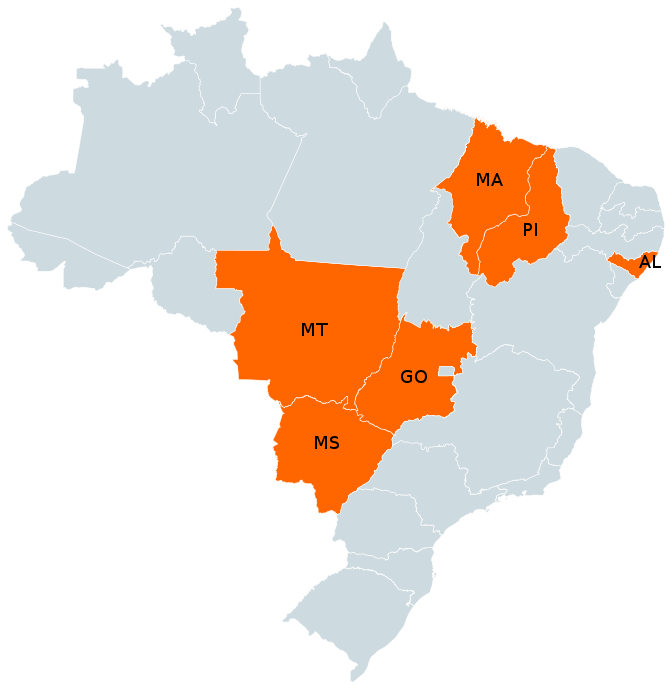
\includegraphics[width=0.6\textwidth]{figuras/mapa-vms.png}
 \caption{PoPs da RNP onde estão alocadas as VMs da CAFe Expresso}
 \label{fig_9}
\end{figure}

O sistema operacional da máquina virtual já estava instalada, é uma imagem básica somente com o serviço de \ac{SSH} disponível. O processo de instalação está descrito na wiki\footnote{https://wiki.rnp.br/pages/viewpage.action?pageId=69963897} da RNP, onde também se encontra o processo de configuração recomendado e que foi realizado para estas máquinas virtuais.

Conforme orientação, é necessário a instalação e configuração de um firewall, para bloquear portas de acesso e liberar somente as utilizadas pelos serviços essenciais, e para reforçar a segurança das máquinas virtuais e evitando ataques e acessos indesejados. Alguns serviços são sensíveis a hora, como os elementos Shibboleth, sendo que cada requisição HTTPS informa também um TIMESTAMP (com o horário da requisição) para calcular um tempo de \textit{timeout} padrão, caso haja falta de interação na sessão aberta pelo usuário, para satisfazer isto, foi instalado o serviço NTP que sincroniza o relógio do servidor com um servidor \acs{NTP} previamente configurado, neste caso foi utilizado o \textit{pool} do NIC.br\footnote{http://www.ntp.br/}. Para gerenciamento dos logs gerados pelos serviços e \textit{debug} do sistema também foi ativo a rotação de logs para compactação automática de logs com data maior que uma semana.

\subsection{Identity Provider - IdP}
\label{ss_c4_inst_idp}

O provedor de identidade é responsável por manter as informações sobre as pessoas vinculadas a uma instituição. Estas informações incluem; Nome, Data de nascimento, Filiação, Sexo, CPF, entre outros. Assim como os tipos de informações internas; Data de admissão, Cargo ocupado, Matrícula, Contato telefônico, Vínculo que as pessoas possuem com a instituição, estudante, técnico administrativo, professor e outros. O IdP estabele seu métod de autenticação interno e deve garantir que cada pessoa tenha um identificador único \cite{moreira:11}.

Para implantação do IdP são necessários alguns softwares e serviços adicionais. Na tabela \ref{tab_2} é possível verificar os requisitos de \textit{software} necessários para implantação do IdP.

\begin{table}[!htpb]
   \begin{small}
	\centering
	\begin{tabular}{|c|c|c|} \hline
		Software & Versão utilizada & Fornecedor \\ \hline
		IdP Shibboleth & 2.1.5 e 2.4.0 & Internet2\\ \hline
		OpenJDK & 6b31-1 & Oracle\\ \hline
		Apache & 2.2.22 & Apache Software Foundation\\ \hline
		Tomcat & 6.0.35 & Apache Software Foundation\\ \hline
		OpenLDAP & 2.4.28 & OpenLDAP Foundation\\ \hline
		OpenSSL & 1.0.1 & OpenSSL Project\\ \hline
	\end{tabular}
	\caption{Requisitos de \textit{software} para implantação do IdP.}
	\label{tab_2} 	
  \end{small}
\end{table}

Para a instalação do IdP é necessário diversos procedimentos, configurações de arquivos, de serviços, sendo um processo complexo e demorado. Neste trabalho foi utilizado a documentação gerada pela RNP disponível na wiki\footnote{https://wiki.rnp.br/display/cafewebsite/Roteiro+de+Atividades+para+Entrada+de+um+IDP}. Este processo foi simplificado para a configuração das máquinas virtuais que foram disponibilizadas, para que os pesquisadores não precisassem se preocupar com a instalação do IdP Shibboleth, esta documentação também está disponibilizada na wiki do Gid Lab\footnote{https://wiki.rnp.br/display/gidlab/Procedimentos+operacionais+da+CAFe+Expresso}.

Na imagem abaixo é possível ver como fica o encapsulamento dos serviços envolvidos para prover o IdP Shibboleth. 

\begin{figure}[!htpb]
 \centering
 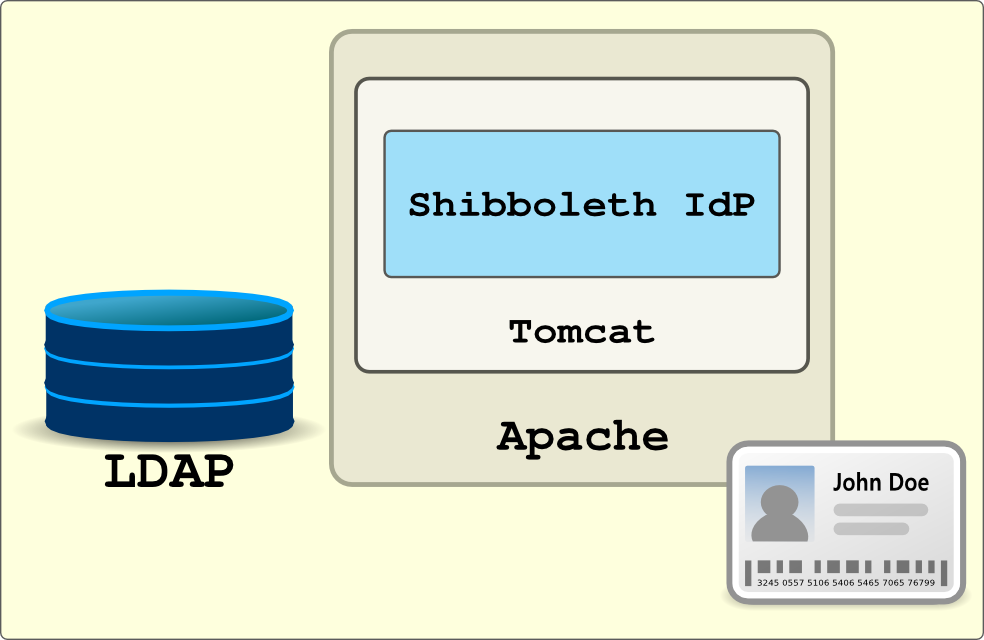
\includegraphics[width=0.5\textwidth]{figuras/vm-idp.png}
 \caption{Encapsulamento dos serviços envolvidos para prover o IdP Shibboleth}
 \label{fig_10}
\end{figure}

O servidor Apache, é responsável por interpretar as requisições HTTP do navegador do usuário e por suportar o Tomcat, o container Java, que permite a execução troca de mensagens e faz a interface entre as requisições HTTP e o Shibboleth IdP. O Shibboleth IdP é uma aplicação Java com componentes em C. É possível utilizar outros \textit{containers}, como Jetty\footnote{http://download.eclipse.org/jetty/}. O LDAP é responsável por armazenar as informações dos usuários e é consultado pelo IdP sempre que este recebe uma solicitação de autenticação.

\subsection{Service Provider - SP}
\label{ss_c4_inst_sp}

O provedor de serviço é responsável por fazer a autorização do usuário e disponibilizar o acesso ao recurso que o usuário deseja através da autenticação e dos atributos disponibilizados pelo IdP. 

A instalação padrão de um Provedor de Serviço é baseada no Shibboleth SP, o foco do SP é proteger a aplicação desenvolvida pelo pesquisador. O processo consiste na instalação de dois elementos:

\begin{itemize}
 \item mod\_shib -- módulo do Apache, responsável por controlar a autorização e o acesso ao recurso;
 \item shibd -- daemon (serviço), responsável por intermediar a solicitação de autenticação e de atributos \cite{moreira:11}.
\end{itemize}

\begin{table}[!htpb]
   \begin{small}
	\centering
	\begin{tabular}{|c|c|c|} \hline
		Software & Versão utilizada & Fornecedor \\ \hline
		SP Shibboleth & 2.4.3 & Internet2\\ \hline
		Apache com módulo Shibboleth & 2.2.22 & Apache Software Foundation\\ \hline
		OpenSSL & 1.0.1 & OpenSSL Project\\ \hline
	\end{tabular}
	\caption{Requisitos de \textit{software} para implantação do SP.}
	\label{tab_3}
  \end{small}
\end{table}

Na figura \ref{fig_11} é possível visualizar como é o encapsulamento dos serviços envolvidos para provimento do SP Shibboleth.

\begin{figure}[!htpb]
 \centering
 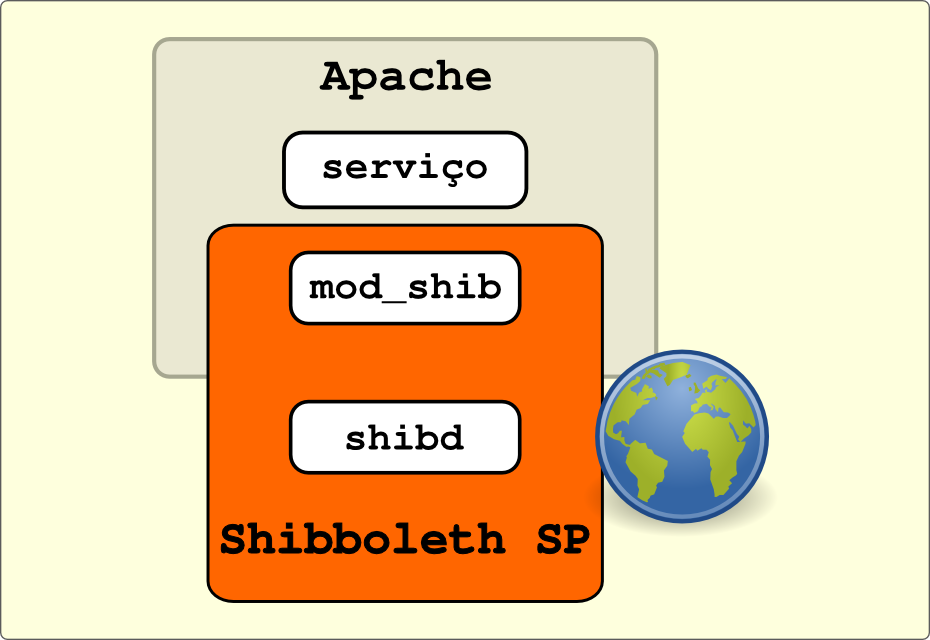
\includegraphics[width=0.5\textwidth]{figuras/vm-sp.png}
 \caption{Encapsulamento dos serviços envolvidos para prover o SP Shibboleth}
 \label{fig_11}
\end{figure}

Assim como o IdP, o processo de instalação do SP também foi usado a documentação gerada pela RNP disponível no link\footnote{https://wiki.rnp.br/display/cafewebsite/Roteiro+de+Atividades+para+Entrada+de+um+SP} e simplificado para que pesquisadores só se preocupasse com algumas configurações específicas referentes ao serviço e o \textit{host} (ou nome) que irá responder ao navegador. O procedimentos para configuração do SP da CAFe Expresso podem ser obtidos na wiki do Gid Lab\footnote{https://wiki.rnp.br/display/gidlab/Procedimentos+operacionais+da+CAFe+Expresso}.

Para ambos os elementos, é necessário gerar um certificado digital para identificação única, garantindo assim a segurança de cada provedor, seja de Identidade como de Serviço. No trabalho foram utilizados certificados auto-assinados.

\subsection{Serviços adicionais}
\label{ss_c4_servicos_add}

Além dos elementos IdP e SP, é possível agregar a estes primeiros alguns serviços. Porém, só IdP e SP não resolvem todo o ambiente, é necessário também um serviço que oferece ao usuário uma lista de IdP’s, onde um destes é o IdP de origem do usuário, esse serviço é o WAYF. Os outros serviços oferecidos pela Federação são: o Embedded DS, que é um serviço similar ao WAYF, porém é nativo no Shibboleth e o uApprove, um serviço que informa aos usuários quais atributos estão sendo solicitados e liberados para o SP, possibilitando ao usuário a liberação destes atributos ou não para o SP. Antes de descrever os serviços WAYF e Embedded DS, será introduzido o propósito geral de ambos os serviços.

O padrão SAML possui um protocolo para descoberta de serviços, DS (Discovery Service), que possibilita a descoberta de provedores de serviços e de identidades.

\subsubsection{WAYF}

O WAYF é responsável por identificar qual é provedor de identidade do usuário. Quando o usuário tenta acessar um recurso disponibilizado por um provedor de serviço da federação, é redirecionado para o WAYF para que possa indicar o seu provedor de identidade e proceder corretamente com a autenticação \cite{moreira:11}

O objetivo do serviço WAYF é enviar o usuário para seu provedor de identidades de origem. A especificação SAML tem descrita quais são os requisitos para se implementar um serviço de descoberta (Discovery Service). No entanto, WAYF e DS podem ser usados como sinônimos, mas WAYF implementa o protocolo DS, com algumas diferenças.

Basicamente, WAYF ou DS, tem somente o propósito de apresentar para o usuário uma lista de provedores de identidades e redirecionar o navegador web para o IdP selecionado e depois retornando para o provedor de serviço. A diferença entre os WAYF e o protocolo DS pode ser vista na figura \ref{fig_12}.

\begin{figure}[!htp]
 \centering
 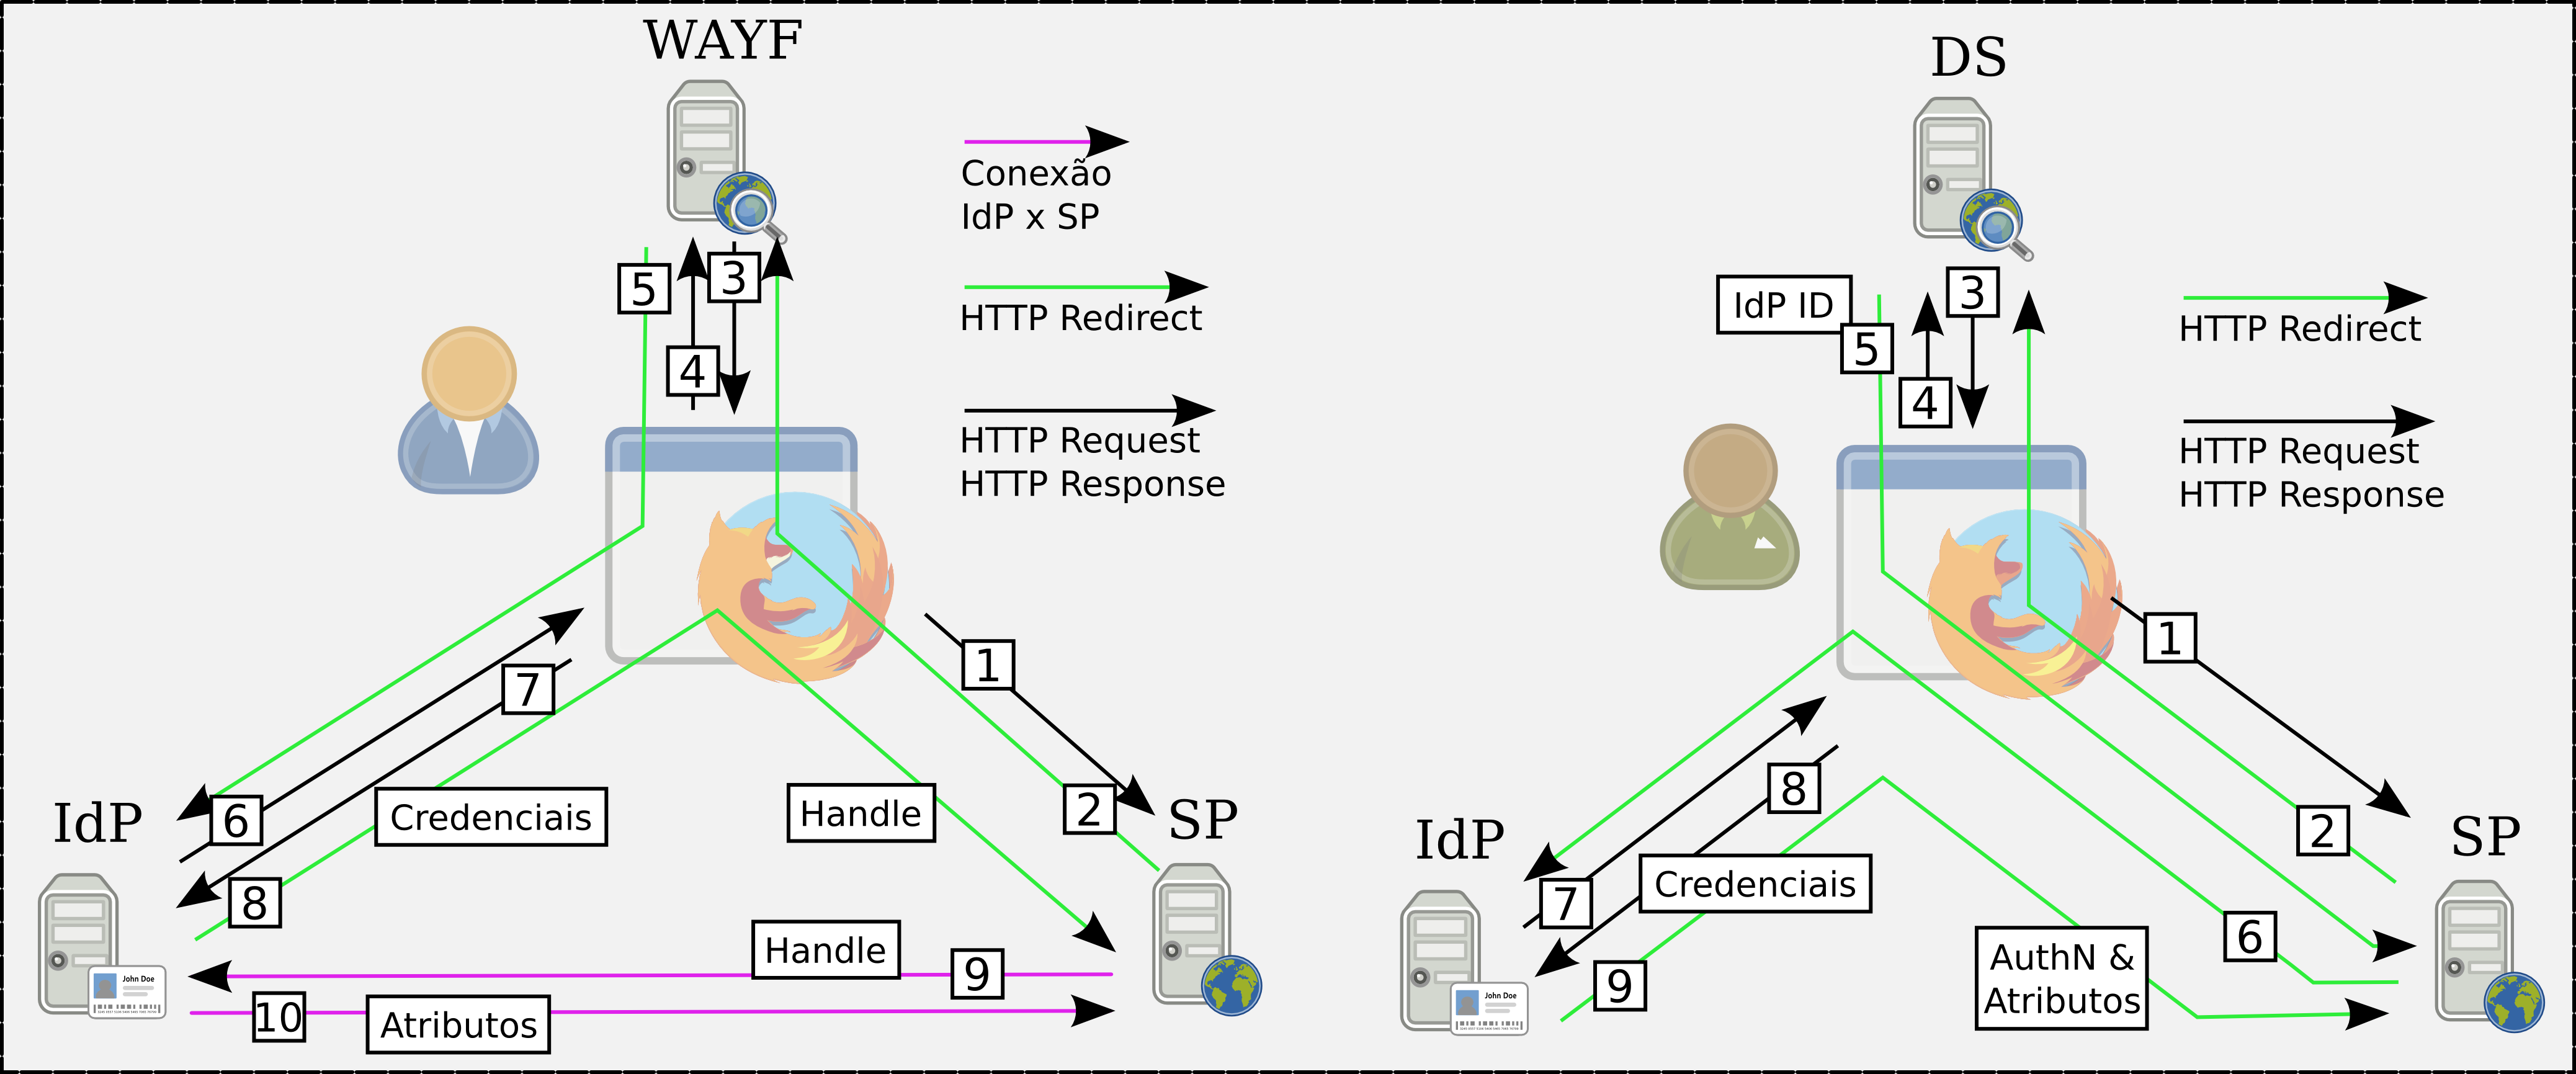
\includegraphics[width=1\textwidth]{figuras/wayf-ds.png}
 \caption{Diferenças entre fluxo de mensagens do WAYF e DS}
 \label{fig_12}
\end{figure}

A implementação desenvolvida pela SWITCH\footnote{https://www.switch.ch/aai} foi feita em PHP que permite suporte a muitos idiomas, diversas formas de selecionar um provedor de identidade, permite fácil atualização de metadados para inclusão de novos provedores na federação.

Algumas características podem ser citadas:
\begin{itemize}
  \item \textit{Open Source} disponibilizado sob licença BSD;
  \item Leitura de metadados SAML2;
  \item Redirecionamento automático para o IdP selecionado na sessão ativa do navegador;
  \item Implementação de um WAYF embarcado.
\end{itemize}


A SWITCH usa a própria implementação WAYF na sua federação a SWITCHaai, e para testes usados por outras federações. Existem outras alternativas que implementam o protocolo DS. Uma dessas é a implementação desenvolvida pela Internet e está descrita logo em seguida. A outra implementação não foi disponibilizada na CAFe Expresso, mas é desenvolvida e mantida pela GRNET\footnote{http://www.grnet.gr/} criado em 2009 e implementado usando Python usando o \textit{framework} Django.identidade do usuário. Quando o usuário tenta aceesar um recuro disponibilizado por um provedor de serviço da federação, ele é redirecionado para o WAYF para que possa indicar o seu provedor de identidade e proceder corretamente com a autenticação \cite{moreira:11}.

\subsubsection{Embedded Discovery Service}

Desenvolvido pela equipe de desenvolvimento do projeto Shibboleth, o Embedded DS pode ser facilmente implementado ao SP Shibboleth. A grande diferença entre o EDS e o WAYF é que para o usuário o processo de redirecionamento é transparente. Ou seja, o SP possui um applet dentro da própria página que permite ao usuário a escolha do seu IdP de origem, é como se ele não saísse da página do serviço.

Outra característica do EDS é prover uma forma fácil de disponibilizar para um SP o protocolo DS embutido direto no próprio SP. Isso permite que a rede se descentralize mais. O elemento DS está presente, e sempre necessitará de um servidor próprio para o mesmo. Pois ele é responsável por fazer o intermédio entre IdP e SP, constituindo a relação de confiança entre estes, sendo assim pode-se dizer que o DS se torna a terceira parte confiante, num ambiente federado.

A wiki do Shibboleth\footnote{https://wiki.shibboleth.net/confluence/display/DEV/EDSDetails}, desenvolvedor oficial do EDS, cita dois principais objetivos do EDS:

\begin{itemize}
  \item Melhorar a experiência durante o processo de login do usuário;
  \item Disponibilizar um DS embutido para SP de forma fácil.
\end{itemize}

De acordo com a wiki\footnote{https://wiki.shibboleth.net} do projeto Shibboleth, onde podem ser encontrados procedimentos de instalação, configuração e relatos do desenvolvimento do \textit{framework} Shibboleth, algumas recomendações são dadas referente a como melhorar a experiência do usuário durante o processo de login, estas recomendações tratam do processo inicial, o botão de login, a localização deste dentro do \textit{layout} da página \textit{web} fazendo a referência somente ao processo de identificação e não à federação. Outras recomendações são sobre a página de seleção do IdP, o painel de IdPs preferidos, entre outras recomendações.

A equipe de desenvolvimento do Shibboleth simplificou a implementação do EDS na página do SP. O EDS é composto basicamente por dois arquivos em Javascript, que tratam os metadados extraindo as informações necessárias de cada IdP para exibição e um \ac{CSS} que define um ID específico para um componente <div> que será agregado ao arquivo HTML da página do SP.

\subsubsection{uApprove}

O uApprove\footnote{https://www.switch.ch/aai/support/tools/uApprove.html} é uma extensão para o IdP Shibboleth desenvolvido pela SWITCH\footnote{http://www.switch.ch/} que possibilita ao usuário saber quais atributos estão sendo liberados para os SP que deseja acessar e permitir que o usuário permita ou não a liberação destes atributos para o SP. Assegurando a aceitação dos Termos de Uso e dos consentimento da liberação dos atributos.

Este processo tem como objetivo os seguintes propósitos:

\begin{itemize}
	\item O usuário é informado sobre a liberação dos seus dados (atributos) para um SP quando acessa o SP pela primeira vez ou seus dados sofreram alterações;
	\item O administrador de um IdP:
	\subitem -- Pode perguntar ao usuário se este aceita os termos de uso antes de acessar qualquer serviço;
	\subitem -- Possui uma ferramenta que implementa leis de proteção de dados ao força o consentimento do usuário antes de dados pessoais dos usuários sejam liberados para um SP;
	\subitem -- Tem controle sobre quando um usuário deu permissões para acesso e quais atributos foi liberado para um determinado SP.
\end{itemize}

Do ponto de vista do usuário, o uApprove é uma aplicação do IdP, onde:
\begin{itemize}
	\item Ele pode aceitar ou negar o termo de uso do IdP Shibboleth num primeiro acesso ao sistema (esta configuração pode ser desabilitada);
	\item Pode aceitar liberar todos os atributo para qualquer SP, sempre que este ou outro SP solicitar;
	\item Deve aceitar para liberer seus atributos num primeiro acesso à um SP (se a liberação de todos os atributos não foi aprovada).
\end{itemize}

O uApprove não permite escolher quais atributos serão liberados, somente se serão ou não liberados para o SP que o usuário está tentando acessar. Na figura \ref{fig_13} é possível visualizar como é o fluxo do uApprove, quais condições são necessárias para que ele se mostre e permita ao usuário visualizar os atributos que estão sendo liberados assim como o Termo de Uso do IdP de origem do usuário.

\begin{figure}[!ht]
 \centering
 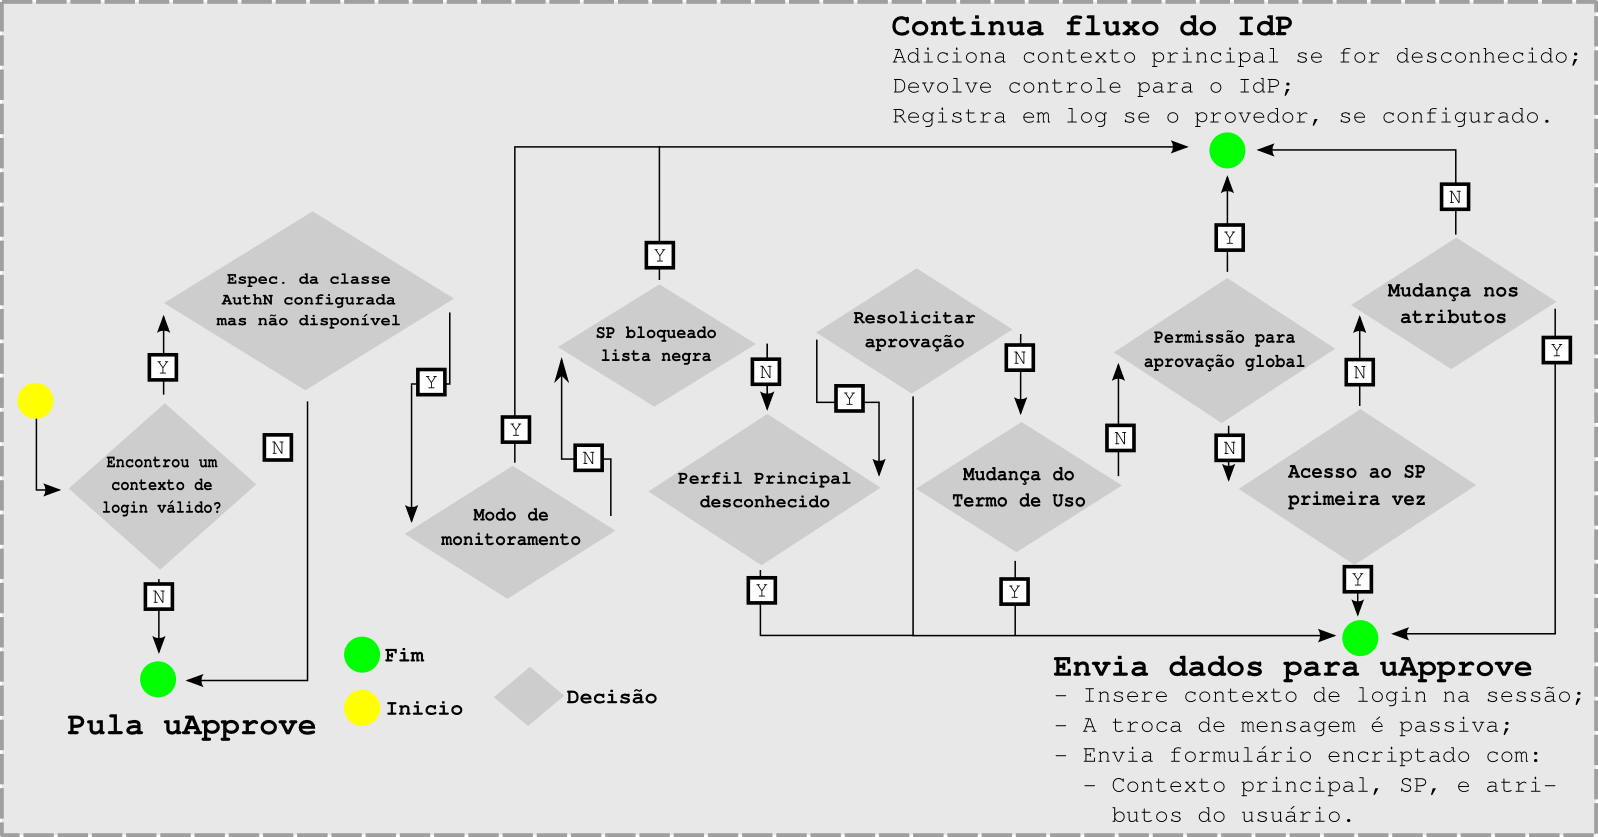
\includegraphics[width=1\textwidth]{figuras/fluxo-uapprove.png}
 \caption{Fluxo de mensagem que definem o funcionamento do uApprove}
 \label{fig_13}
\end{figure}

Como o uApprove é um \textit{plug-in} para o IdP é necssário configurá-lo como tal, inserir as chamadas do uApprove dentro das configurações do IdP possibilitando que o primeiro possa interceptar o fluxo normal do IdP e verificar se o usuário possui um contexto de login válido, para então obter os atributos e mostrar na tela do usuário o que está sendo solicitado pelo SP e o que está sendo liberado dos atributos solicitados. Ao término do fluxo, se o usuário aceitar o Termo de Uso e aprovar a liberação dos atributos, o uApprove regitra esta interação no banco de dados. Caso tenha alterações no Termo de Uso ou mais atributos sejam liberados para o usuário o uApprove verifica estas informações novamente e solicita novo consentimento do usuário.

O requisitos de \textit{software} para instalação do \textit{uApprove} estão listados na tabela \ref{tab_4}.

\begin{table}[!htpb]
   \begin{small}
	\centering
	\begin{tabular}{|c|c|c|} \hline
		Software & Versão utilizada & Fornecedor \\ \hline
		IdP Shibboleth & 2.4.0 & Internet2\\ \hline
		uApprove & 2.5 & SWITCHaai\\ \hline
		MySQL & 5.5.37 & Oracle\\ \hline
		MySQL JDBC Connector & 2.5.25 & Oracle\\ \hline
	\end{tabular}
	\caption{Requisitos de \textit{software} para implantação do uApprove.}
	\label{tab_4}  	
  \end{small}
\end{table}

O uApprove proporciona algumas funcionalidades, permite que o usuário limpe os atributos liberados anteriormente e força que o uApprove verifique novamente as informações dos atributos do usuário que estão sendo solicitados pelo SP. Além disto, o administrador do IdP que tenha o uApprove, pode habilitar que em casos de falha de conexão com Banco de Dados, o uApprove, haja como se estivesse realizando o registro das informações liberadas pelo usuário, no entanto a aprovação do consentimento do usuário não será registrada no banco, mas mostrará ao usuário os dados solicitados pelo SP, no entanto num próximo login, para aquele SP será solicitado novamente consentimento de liberação de atributos do usuário.
% ----------------------------------------------------------------------- %
% Arquivo: conclusoes.tex
% ----------------------------------------------------------------------- %
\chapter{Conclusões}
\label{c_conclusao}

O crescimento da internet, como meio para realização de negócios, estudos, trocas de informações de forma geral, entre Homem X Máquina (\textit{Human to Machine} -- H2M) e Máquina X Máquina (\textit{Machine to Machine} -- M2M), criou uma necessidade natural de identificação das entidades que convivem na rede de computadores. Uma necessidade que é tratada no processo de gestão de identidades, por meio de divermos modelos.

O conceito de Gestão de Identidades Federada têm crescido nos últimos anos e refere-se a um conjunto de tecnologias e padrões que permite a interação do usuário com diversos serviços usando apenas uma credencial de acesso. A função básica da identidade federada, o SSO, possibilita ao usuário o uso da autenticação feita em um \textit{site} e o uso desta mesma validação para acessar outros serviços protegidos \cite{kallela:08}.

No trabalho em questão, foi abordado o modelo de gestão de identidades federadas, como implementado no \textit{framework} Shibboleth. Este modelo permite a descentralização dos provedores de identidade dos provedores de serviço, que além de facilitar o gerenciamento da infraestrutura dos provedores, para os administradores destes, também facilita para o usuário que precisará de somente uma única identificação para acesso aos serviços disponibilizados pelos provedores de serviço. No modelo de gestão de identidades federadas a especificação mais utilizada é o SAML, que define que tipos de informações são trocadas pelos provedores de identidades e de  serviços. O \textit{framework} Shibboleth é o mais utilizado em ambientes acadêmicos.

Gestão de Identidades federadas é uma área ativa de pesquisa, sendo que muitos trabalhos desenvolvidos nesta área precisam realizar experimentos com soluções e frameworks consolidados como o Shibboleth. Desenvolver pesquisas aplicadas na área de gestão de identidades federadas exige que os experimentos sejam conduzidos em um ambiente que implemente uma federação em sua totalidade. Configurar uma federação  para realizar experimentos de uma pesquisa, pode ser uma tarefa mais árdua e demorada do que a implementação da pesquisa propriamente dita \cite{wangham:13}.

O objetivo deste trabalho era implantar uma parte do GId Lab, um ambiente virtual de apoio aos pesquisadores brasileiros a fim de estimular e facilitar o desenvolvimento de novas soluções que possam vir a ser disponibilizadas na federação acadêmica, CAFe, ou como um serviço da RNP. Do objetivo proposto no início do trabalho, todas as atividades foram realizadas. De uma forma geral, a implantação da federação acadêmica foi realizada em sua plenitude, o ambiente é composto de três Provedores de Identidade \ac{IdP}, três Provedores de Serviço \ac{SP}, dois serviços de descoberta, o \ac{WAYF} e o \ac{EDS} e um serviço que solicita o consentimento do usuário para liberação dos atributos solicitados pelo \ac{SP} ao IdP, o \textit{uApprove}. Além disto, foram disponibilizadas máquinas virtuais para \textit{download} por pesquisadores interessados em implantar uma federação Shibboleth. Duas categorias de máquinas virtuais foram disponibilizadas, é possível realizar \textit{download} dos elementos Shibboleth, separadamente, para fazer testes na CAFe Expresso, ou uma federação completa para uso local.

Para trabalhos futuros podem ser sugeridos a implantação do IdP+, que é um IdP para tradução de credenciais de segurança, permitindo a geração de certificados X.509 e permitindo que aplicações não \textit{web} possam fazer uso de autenticação federadas Shibboleth. Outra sugestão para trabalhos futuros é a implantação do \ac{SGC} que permite a tradução de credenciais Shibboleth em certificados digitais, que podem ser consumidas por serviços que requerem estes tipos de certificados. Mais uma sugestão de trabalho futuro é a implementação do \ac{SLO}. Atualmente a forma de se deslogar de uma sessão federada, é fechar o navegador \textit{web}, com o \ac{SLO} seria possível finalizar a sessão com um único clique. No entanto esta funcionalidade não é totalmente suportada pelo \textit{framework} Shibboleth, e só será na próxima versão, que não tem previsão de lançamento oficial. Uma última sugestão de trabalhos futuros é integração entre a federação CAFe Expresso, que utiliza a especificação SAML através do \textit{framework} Shibboleth e outras tecnologias de gestão de identidade federada, como OAuth\footnote{http://oauth.net/} e OpenID Connect\footnote{http://openid.net/} que implementam outros padrões de comunicação, diferentes do SAML.

% inclusão de apêndices (se houver)
% \apendice
% \include{apendice1}

% inclusão de anexos (se houver)
% \anexo
% \include{anexo1}

\bibliographystyle{abnt-alf}
\bibliography{referencias}

\end{document}
